
%% bare_adv.tex
%% V1.4
%% 2012/12/27
%% by Michael Shell
%% See: 
%% http://www.michaelshell.org/
%% for current contact information.
%%
%% This is a skeleton file demonstrating the advanced use of IEEEtran.cls
%% (requires IEEEtran.cls version 1.8 or later) with an IEEE Computer
%% Society journal paper.
%%
%% Support sites:
%% http://www.michaelshell.org/tex/ieeetran/
%% http://www.ctan.org/tex-archive/macros/latex/contrib/IEEEtran/
%% and
%% http://www.ieee.org/

%%*************************************************************************
%% Legal Notice:
%% This code is offered as-is without any warranty either expressed or
%% implied; without even the implied warranty of MERCHANTABILITY or
%% FITNESS FOR A PARTICULAR PURPOSE! 
%% User assumes all risk.
%% In no event shall IEEE or any contributor to this code be liable for
%% any damages or losses, including, but not limited to, incidental,
%% consequential, or any other damages, resulting from the use or misuse
%% of any information contained here.
%%
%% All comments are the opinions of their respective authors and are not
%% necessarily endorsed by the IEEE.
%%
%% This work is distributed under the LaTeX Project Public License (LPPL)
%% ( http://www.latex-project.org/ ) version 1.3, and may be freely used,
%% distributed and modified. A copy of the LPPL, version 1.3, is included
%% in the base LaTeX documentation of all distributions of LaTeX released
%% 2003/12/01 or later.
%% Retain all contribution notices and credits.
%% ** Modified files should be clearly indicated as such, including  **
%% ** renaming them and changing author support contact information. **
%%
%% File list of work: IEEEtran.cls, IEEEtran_HOWTO.pdf, bare_adv.tex,
%%                    bare_conf.tex, bare_jrnl.tex, bare_jrnl_compsoc.tex,
%%                    bare_jrnl_transmag.tex
%%*************************************************************************

% *** Authors should verify (and, if needed, correct) their LaTeX system  ***
% *** with the testflow diagnostic prior to trusting their LaTeX platform ***
% *** with production work. IEEE's font choices can trigger bugs that do  ***
% *** not appear when using other class files.                            ***
% The testflow support page is at:
% http://www.michaelshell.org/tex/testflow/



% IEEEtran V1.7 and later provides for these CLASSINPUT macros to allow the
% user to reprogram some IEEEtran.cls defaults if needed. These settings
% override the internal defaults of IEEEtran.cls regardless of which class
% options are used. Do not use these unless you have good reason to do so as
% they can result in nonIEEE compliant documents. User beware. ;)
%
%\newcommand{\CLASSINPUTbaselinestretch}{1.0} % baselinestretch
%\newcommand{\CLASSINPUTinnersidemargin}{1in} % inner side margin
%\newcommand{\CLASSINPUToutersidemargin}{1in} % outer side margin
%\newcommand{\CLASSINPUTtoptextmargin}{1in}   % top text margin
%\newcommand{\CLASSINPUTbottomtextmargin}{1in}% bottom text margin



% Note that the a4paper option is mainly intended so that authors in
% countries using A4 can easily print to A4 and see how their papers will
% look in print - the typesetting of the document will not typically be
% affected with changes in paper size (but the bottom and side margins will).
% Use the testflow package mentioned above to verify correct handling of
% both paper sizes by the user's LaTeX system.
%
% Also note that the "draftcls" or "draftclsnofoot", not "draft", option
% should be used if it is desired that the figures are to be displayed in
% draft mode.
%
\documentclass[12pt,journal,compsoc]{IEEEtran}
% The Computer Society requires 12pt.
% If IEEEtran.cls has not been installed into the LaTeX system files,
% manually specify the path to it like:
% \documentclass[10pt,journal,compsoc]{../sty/IEEEtran}


% For Computer Society journals, IEEEtran defaults to the use of 
% Palatino/Palladio as is done in IEEE Computer Society journals.
% To go back to Times Roman, you can use this code:
%\renewcommand{\rmdefault}{ptm}\selectfont





% Some very useful LaTeX packages include:
% (uncomment the ones you want to load)



% *** MISC UTILITY PACKAGES ***
%
%\usepackage{ifpdf}
% Heiko Oberdiek's ifpdf.sty is very useful if you need conditional
% compilation based on whether the output is pdf or dvi.
% usage:
% \ifpdf
%   % pdf code
% \else
%   % dvi code
% \fi
% The latest version of ifpdf.sty can be obtained from:
% http://www.ctan.org/tex-archive/macros/latex/contrib/oberdiek/
% Also, note that IEEEtran.cls V1.7 and later provides a builtin
% \ifCLASSINFOpdf conditional that works the same way.
% When switching from latex to pdflatex and vice-versa, the compiler may
% have to be run twice to clear warning/error messages.






% *** CITATION PACKAGES ***
%
\ifCLASSOPTIONcompsoc
  % IEEE Computer Society needs nocompress option
  % requires cite.sty v4.0 or later (November 2003)
  % \usepackage[nocompress]{cite}
\else
  % normal IEEE
  % \usepackage{cite}
\fi
% cite.sty was written by Donald Arseneau
% V1.6 and later of IEEEtran pre-defines the format of the cite.sty package
% \cite{} output to follow that of IEEE. Loading the cite package will
% result in citation numbers being automatically sorted and properly
% "compressed/ranged". e.g., [1], [9], [2], [7], [5], [6] without using
% cite.sty will become [1], [2], [5]--[7], [9] using cite.sty. cite.sty's
% \cite will automatically add leading space, if needed. Use cite.sty's
% noadjust option (cite.sty V3.8 and later) if you want to turn this off
% such as if a citation ever needs to be enclosed in parenthesis.
% cite.sty is already installed on most LaTeX systems. Be sure and use
% version 4.0 (2003-05-27) and later if using hyperref.sty. cite.sty does
% not currently provide for hyperlinked citations.
% The latest version can be obtained at:
% http://www.ctan.org/tex-archive/macros/latex/contrib/cite/
% The documentation is contained in the cite.sty file itself.
%
% Note that some packages require special options to format as the Computer
% Society requires. In particular, Computer Society  papers do not use
% compressed citation ranges as is done in typical IEEE papers
% (e.g., [1]-[4]). Instead, they list every citation separately in order
% (e.g., [1], [2], [3], [4]). To get the latter we need to load the cite
% package with the nocompress option which is supported by cite.sty v4.0
% and later.
%
% Note also the use of a CLASSOPTION conditional provided by 
% IEEEtran.cls V1.7 and later.





% *** GRAPHICS RELATED PACKAGES ***
%
\ifCLASSINFOpdf
  \usepackage[pdftex]{graphicx}
  % declare the path(s) where your graphic files are
  \graphicspath{{/home/saf537/Documents/CUSP/Capstone/Bus-Capstone/plots}}
  % and their extensions so you won't have to specify these with
  % every instance of \includegraphics
  \DeclareGraphicsExtensions{.pdf,.jpeg,.png,.jpg,.PNG}
\else
  % or other class option (dvipsone, dvipdf, if not using dvips). graphicx
  % will default to the driver specified in the system graphics.cfg if no
  % driver is specified.
  \usepackage[dvips]{graphicx}
  % declare the path(s) where your graphic files are
  \graphicspath{{/home/saf537/Documents/CUSP/Capstone/Bus-Capstone/plots}}
  % and their extensions so you won't have to specify these with
  % every instance of \includegraphics
  % \DeclareGraphicsExtensions{.eps}
\fi
% graphicx was written by David Carlisle and Sebastian Rahtz. It is
% required if you want graphics, photos, etc. graphicx.sty is already
% installed on most LaTeX systems. The latest version and documentation
% can be obtained at: 
% http://www.ctan.org/tex-archive/macros/latex/required/graphics/
% Another good source of documentation is "Using Imported Graphics in
% LaTeX2e" by Keith Reckdahl which can be found at:
% http://www.ctan.org/tex-archive/info/epslatex/
%
% latex, and pdflatex in dvi mode, support graphics in encapsulated
% postscript (.eps) format. pdflatex in pdf mode supports graphics
% in .pdf, .jpeg, .png and .mps (metapost) formats. Users should ensure
% that all non-photo figures use a vector format (.eps, .pdf, .mps) and
% not a bitmapped formats (.jpeg, .png). IEEE frowns on bitmapped formats
% which can result in "jaggedy"/blurry rendering of lines and letters as
% well as large increases in file sizes.
%
% You can find documentation about the pdfTeX application at:
% http://www.tug.org/applications/pdftex


\usepackage{fancyhdr}
\usepackage{lastpage}
\usepackage{biblatex}
\usepackage{url}
\usepackage{hyperref}
\usepackage{graphicx, wrapfig, subcaption, setspace, booktabs}
\usepackage[T1]{fontenc}
\usepackage[font=small, labelfont=bf]{caption}
\usepackage{fourier}
\usepackage[protrusion=true, expansion=true]{microtype}
\usepackage[english]{babel}
%\usepackage{sectsty}
\usepackage{url, lipsum}


% *** MATH PACKAGES ***
%
%\usepackage[cmex10]{amsmath}
% A popular package from the American Mathematical Society that provides
% many useful and powerful commands for dealing with mathematics. If using
% it, be sure to load this package with the cmex10 option to ensure that
% only type 1 fonts will utilized at all point sizes. Without this option,
% it is possible that some math symbols, particularly those within
% footnotes, will be rendered in bitmap form which will result in a
% document that can not be IEEE Xplore compliant!
%
% Also, note that the amsmath package sets \interdisplaylinepenalty to 10000
% thus preventing page breaks from occurring within multiline equations. Use:
%\interdisplaylinepenalty=2500
% after loading amsmath to restore such page breaks as IEEEtran.cls normally
% does. amsmath.sty is already installed on most LaTeX systems. The latest
% version and documentation can be obtained at:
% http://www.ctan.org/tex-archive/macros/latex/required/amslatex/math/





% *** SPECIALIZED LIST PACKAGES ***
%\usepackage{acronym}
% acronym.sty was written by Tobias Oetiker. This package provides tools for
% managing documents with large numbers of acronyms. (You don't *have* to
% use this package - unless you have a lot of acronyms, you may feel that
% such package management of them is bit of an overkill.)
% Do note that the acronym environment (which lists acronyms) will have a
% problem when used under IEEEtran.cls because acronym.sty relies on the
% description list environment - which IEEEtran.cls has customized for
% producing IEEE style lists. A workaround is to declared the longest
% label width via the IEEEtran.cls \IEEEiedlistdecl global control:
%
% \renewcommand{\IEEEiedlistdecl}{\IEEEsetlabelwidth{SONET}}
% \begin{acronym}
%
% \end{acronym}
% \renewcommand{\IEEEiedlistdecl}{\relax}% remember to reset \IEEEiedlistdecl
%
% instead of using the acronym environment's optional argument.
% The latest version and documentation can be obtained at:
% http://www.ctan.org/tex-archive/macros/latex/contrib/acronym/


%\usepackage{algorithmic}
% algorithmic.sty was written by Peter Williams and Rogerio Brito.
% This package provides an algorithmic environment fo describing algorithms.
% You can use the algorithmic environment in-text or within a figure
% environment to provide for a floating algorithm. Do NOT use the algorithm
% floating environment provided by algorithm.sty (by the same authors) or
% algorithm2e.sty (by Christophe Fiorio) as IEEE does not use dedicated
% algorithm float types and packages that provide these will not provide
% correct IEEE style captions. The latest version and documentation of
% algorithmic.sty can be obtained at:
% http://www.ctan.org/tex-archive/macros/latex/contrib/algorithms/
% There is also a support site at:
% http://algorithms.berlios.de/index.html
% Also of interest may be the (relatively newer and more customizable)
% algorithmicx.sty package by Szasz Janos:
% http://www.ctan.org/tex-archive/macros/latex/contrib/algorithmicx/




% *** ALIGNMENT PACKAGES ***
%
%\usepackage{array}
% Frank Mittelbach's and David Carlisle's array.sty patches and improves
% the standard LaTeX2e array and tabular environments to provide better
% appearance and additional user controls. As the default LaTeX2e table
% generation code is lacking to the point of almost being broken with
% respect to the quality of the end results, all users are strongly
% advised to use an enhanced (at the very least that provided by array.sty)
% set of table tools. array.sty is already installed on most systems. The
% latest version and documentation can be obtained at:
% http://www.ctan.org/tex-archive/macros/latex/required/tools/


%\usepackage{mdwmath}
%\usepackage{mdwtab}
% Also highly recommended is Mark Wooding's extremely powerful MDW tools,
% especially mdwmath.sty and mdwtab.sty which are used to format equations
% and tables, respectively. The MDWtools set is already installed on most
% LaTeX systems. The lastest version and documentation is available at:
% http://www.ctan.org/tex-archive/macros/latex/contrib/mdwtools/


% IEEEtran contains the IEEEeqnarray family of commands that can be used to
% generate multiline equations as well as matrices, tables, etc., of high
% quality.


%\usepackage{eqparbox}
% Also of notable interest is Scott Pakin's eqparbox package for creating
% (automatically sized) equal width boxes - aka "natural width parboxes".
% Available at:
% http://www.ctan.org/tex-archive/macros/latex/contrib/eqparbox/




% *** SUBFIGURE PACKAGES ***
%\ifCLASSOPTIONcompsoc
%  \usepackage[caption=false,font=normalsize,labelfont=sf,textfont=sf]{subfig}
%\else
%  \usepackage[caption=false,font=footnotesize]{subfig}
%\fi
% subfig.sty, written by Steven Douglas Cochran, is the modern replacement
% for subfigure.sty, the latter of which is no longer maintained and is
% incompatible with some LaTeX packages including fixltx2e. However,
% subfig.sty requires and automatically loads Axel Sommerfeldt's caption.sty
% which will override IEEEtran.cls' handling of captions and this will result
% in non-IEEE style figure/table captions. To prevent this problem, be sure
% and invoke subfig.sty's "caption=false" package option (available since
% subfig.sty version 1.3, 2005/06/28) as this is will preserve IEEEtran.cls
% handling of captions.
% Note that the Computer Society format requires a larger sans serif font
% than the serif footnote size font used in traditional IEEE formatting
% and thus the need to invoke different subfig.sty package options depending
% on whether compsoc mode has been enabled.
%
% The latest version and documentation of subfig.sty can be obtained at:
% http://www.ctan.org/tex-archive/macros/latex/contrib/subfig/




% *** FLOAT PACKAGES ***
%
%\usepackage{fixltx2e}
% fixltx2e, the successor to the earlier fix2col.sty, was written by
% Frank Mittelbach and David Carlisle. This package corrects a few problems
% in the LaTeX2e kernel, the most notable of which is that in current
% LaTeX2e releases, the ordering of single and double column floats is not
% guaranteed to be preserved. Thus, an unpatched LaTeX2e can allow a
% single column figure to be placed prior to an earlier double column
% figure. The latest version and documentation can be found at:
% http://www.ctan.org/tex-archive/macros/latex/base/


%\usepackage{stfloats}
% stfloats.sty was written by Sigitas Tolusis. This package gives LaTeX2e
% the ability to do double column floats at the bottom of the page as well
% as the top. (e.g., "\begin{figure*}[!b]" is not normally possible in
% LaTeX2e). It also provides a command:
%\fnbelowfloat
% to enable the placement of footnotes below bottom floats (the standard
% LaTeX2e kernel puts them above bottom floats). This is an invasive package
% which rewrites many portions of the LaTeX2e float routines. It may not work
% with other packages that modify the LaTeX2e float routines. The latest
% version and documentation can be obtained at:
% http://www.ctan.org/tex-archive/macros/latex/contrib/sttools/
% Do not use the stfloats baselinefloat ability as IEEE does not allow
% \baselineskip to stretch. Authors submitting work to the IEEE should note
% that IEEE rarely uses double column equations and that authors should try
% to avoid such use. Do not be tempted to use the cuted.sty or midfloat.sty
% packages (also by Sigitas Tolusis) as IEEE does not format its papers in
% such ways.
% Do not attempt to use stfloats with fixltx2e as they are incompatible.
% Instead, use Morten Hogholm'a dblfloatfix which combines the features
% of both fixltx2e and stfloats:
%
% \usepackage{dblfloatfix}
% The latest version can be found at:
% http://www.ctan.org/tex-archive/macros/latex/contrib/dblfloatfix/


%\ifCLASSOPTIONcaptionsoff
%  \usepackage[nomarkers]{endfloat}
% \let\MYoriglatexcaption\caption
% \renewcommand{\caption}[2][\relax]{\MYoriglatexcaption[#2]{#2}}
%\fi
% endfloat.sty was written by James Darrell McCauley, Jeff Goldberg and 
% Axel Sommerfeldt. This package may be useful when used in conjunction with 
% IEEEtran.cls'  captionsoff option. Some IEEE journals/societies require that
% submissions have lists of figures/tables at the end of the paper and that
% figures/tables without any captions are placed on a page by themselves at
% the end of the document. If needed, the draftcls IEEEtran class option or
% \CLASSINPUTbaselinestretch interface can be used to increase the line
% spacing as well. Be sure and use the nomarkers option of endfloat to
% prevent endfloat from "marking" where the figures would have been placed
% in the text. The two hack lines of code above are a slight modification of
% that suggested by in the endfloat docs (section 8.4.1) to ensure that
% the full captions always appear in the list of figures/tables - even if
% the user used the short optional argument of \caption[]{}.
% IEEE papers do not typically make use of \caption[]'s optional argument,
% so this should not be an issue. A similar trick can be used to disable
% captions of packages such as subfig.sty that lack options to turn off
% the subcaptions:
% For subfig.sty:
% \let\MYorigsubfloat\subfloat
% \renewcommand{\subfloat}[2][\relax]{\MYorigsubfloat[]{#2}}
% However, the above trick will not work if both optional arguments of
% the \subfloat command are used. Furthermore, there needs to be a
% description of each subfigure *somewhere* and endfloat does not add
% subfigure captions to its list of figures. Thus, the best approach is to
% avoid the use of subfigure captions (many IEEE journals avoid them anyway)
% and instead reference/explain all the subfigures within the main caption.
% The latest version of endfloat.sty and its documentation can obtained at:
% http://www.ctan.org/tex-archive/macros/latex/contrib/endfloat/
%
% The IEEEtran \ifCLASSOPTIONcaptionsoff conditional can also be used
% later in the document, say, to conditionally put the References on a 
% page by themselves.





% *** PDF, URL AND HYPERLINK PACKAGES ***
%
\usepackage{url}
% url.sty was written by Donald Arseneau. It provides better support for
% handling and breaking URLs. url.sty is already installed on most LaTeX
% systems. The latest version and documentation can be obtained at:
% http://www.ctan.org/tex-archive/macros/latex/contrib/url/
% Basically, \url{my_url_here}.


% NOTE: PDF thumbnail features are not required in IEEE papers
%       and their use requires extra complexity and work.
%\ifCLASSINFOpdf
%  \usepackage[pdftex]{thumbpdf}
%\else
%  \usepackage[dvips]{thumbpdf}
%\fi
% thumbpdf.sty and its companion Perl utility were written by Heiko Oberdiek.
% It allows the user a way to produce PDF documents that contain fancy
% thumbnail images of each of the pages (which tools like acrobat reader can
% utilize). This is possible even when using dvi->ps->pdf workflow if the
% correct thumbpdf driver options are used. thumbpdf.sty incorporates the
% file containing the PDF thumbnail information (filename.tpm is used with
% dvips, filename.tpt is used with pdftex, where filename is the base name of
% your tex document) into the final ps or pdf output document. An external
% utility, the thumbpdf *Perl script* is needed to make these .tpm or .tpt
% thumbnail files from a .ps or .pdf version of the document (which obviously
% does not yet contain pdf thumbnails). Thus, one does a:
% 
% thumbpdf filename.pdf 
%
% to make a filename.tpt, and:
%
% thumbpdf --mode dvips filename.ps
%
% to make a filename.tpm which will then be loaded into the document by
% thumbpdf.sty the NEXT time the document is compiled (by pdflatex or
% latex->dvips->ps2pdf). Users must be careful to regenerate the .tpt and/or
% .tpm files if the main document changes and then to recompile the
% document to incorporate the revised thumbnails to ensure that thumbnails
% match the actual pages. It is easy to forget to do this!
% 
% Unix systems come with a Perl interpreter. However, MS Windows users
% will usually have to install a Perl interpreter so that the thumbpdf
% script can be run. The Ghostscript PS/PDF interpreter is also required.
% See the thumbpdf docs for details. The latest version and documentation
% can be obtained at.
% http://www.ctan.org/tex-archive/support/thumbpdf/


% NOTE: PDF hyperlink and bookmark features are not required in IEEE
%       papers and their use requires extra complexity and work.
% *** IF USING HYPERREF BE SURE AND CHANGE THE EXAMPLE PDF ***
% *** TITLE/SUBJECT/AUTHOR/KEYWORDS INFO BELOW!!           ***
\newcommand\MYhyperrefoptions{bookmarks=true,bookmarksnumbered=true,
pdfpagemode={UseOutlines},plainpages=false,pdfpagelabels=true,
colorlinks=true,linkcolor={black},citecolor={black},urlcolor={black},
pdftitle={Bare Demo of IEEEtran.cls for Computer Society Journals},%<!CHANGE!
pdfsubject={Typesetting},%<!CHANGE!
pdfauthor={ },%<!CHANGE!
pdfkeywords={ }}%<^!CHANGE!
%\ifCLASSINFOpdf

\usepackage{amsmath, amsthm, amssymb, amsfonts}
%\usepackage[\MYhyperrefoptions,pdftex]{hyperref}
%\else
%\usepackage[\MYhyperrefoptions,breaklinks=true,dvips]{hyperref}
%\usepackage[•]{•}{breakurl}
%\fi
% One significant drawback of using hyperref under DVI output is that the
% LaTeX compiler cannot break URLs across lines or pages as can be done
% under pdfLaTeX's PDF output via the hyperref pdftex driver. This is
% probably the single most important capability distinction between the
% DVI and PDF output. Perhaps surprisingly, all the other PDF features
% (PDF bookmarks, thumbnails, etc.) can be preserved in
% .tex->.dvi->.ps->.pdf workflow if the respective packages/scripts are
% loaded/invoked with the correct driver options (dvips, etc.). 
% As most IEEE papers use URLs sparingly (mainly in the references), this
% may not be as big an issue as with other publications.
%
% That said, Vilar Camara Neto created his breakurl.sty package which
% permits hyperref to easily break URLs even in dvi mode.
% Note that breakurl, unlike most other packages, must be loaded
% AFTER hyperref. The latest version of breakurl and its documentation can
% be obtained at:
% http://www.ctan.org/tex-archive/macros/latex/contrib/breakurl/
% breakurl.sty is not for use under pdflatex pdf mode.
%
% The advanced features offer by hyperref.sty are not required for IEEE
% submission, so users should weigh these features against the added
% complexity of use.
% The package options above demonstrate how to enable PDF bookmarks
% (a type of table of contents viewable in Acrobat Reader) as well as
% PDF document information (title, subject, author and keywords) that is
% viewable in Acrobat reader's Document_Properties menu. PDF document
% information is also used extensively to automate the cataloging of PDF
% documents. The above set of options ensures that hyperlinks will not be
% colored in the text and thus will not be visible in the printed page,
% but will be active on "mouse over". USING COLORS OR OTHER HIGHLIGHTING
% OF HYPERLINKS CAN RESULT IN DOCUMENT REJECTION BY THE IEEE, especially if
% these appear on the "printed" page. IF IN DOUBT, ASK THE RELEVANT
% SUBMISSION EDITOR. You may need to add the option hypertexnames=false if
% you used duplicate equation numbers, etc., but this should not be needed
% in normal IEEE work.
% The latest version of hyperref and its documentation can be obtained at:
% http://www.ctan.org/tex-archive/macros/latex/contrib/hyperref/





% *** Do not adjust lengths that control margins, column widths, etc. ***
% *** Do not use packages that alter fonts (such as pslatex).         ***
% There should be no need to do such things with IEEEtran.cls V1.6 and later.
% (Unless specifically asked to do so by the journal or conference you plan
% to submit to, of course. )


% correct bad hyphenation here
\hyphenation{ }


\begin{document}
%
% paper title
% can use linebreaks \\ within to get better formatting as desired
% Do not put math or special symbols in the title.
\title{Bus Reliability Metrics using Public MTA Bus Time Data}
%
%
% author names and IEEE memberships
% note positions of commas and nonbreaking spaces ( ~ ) LaTeX will not break
% a structure at a ~ so this keeps an author's name from being broken across
% two lines.
% use \thanks{} to gain access to the first footnote area
% a separate \thanks must be used for each paragraph as LaTeX2e's \thanks
% was not built to handle multiple paragraphs
%
%
%\IEEEcompsocitemizethanks is a special \thanks that produces the bulleted
% lists the Computer Society journals use for "first footnote" author
% affiliations. Use \IEEEcompsocthanksitem which works much like \item
% for each affiliation group. When not in compsoc mode,
% \IEEEcompsocitemizethanks becomes like \thanks and
% \IEEEcompsocthanksitem becomes a line break with idention. This
% facilitates dual compilation, although admittedly the differences in the
% desired content of \author between the different types of papers makes a
% one-size-fits-all approach a daunting prospect. For instance, compsoc 
% journal papers have the author affiliations above the "Manuscript
% received ..."  text while in non-compsoc journals this is reversed. Sigh.

\author{Jiaxu~Zhou,
        Yuqiao~Cen,
        Matthew~Urbanek,
        Bonan~Yuan,
        and~Sara~Arango-Franco}% <-this % stops a space
\IEEEcompsocitemizethanks{\IEEEcompsocthanksitem Center for Urban Science and Progress, New York University.\protect\\
% note need leading \protect in front of \\ to get a newline within \thanks as
% \\ is fragile and will error, could use \hfil\break instead.
}% <-this % stops a space
%\thanks{Manuscript received April 19, 2005; revised December 27, 2012.}

% note the % following the last \IEEEmembership and also \thanks - 
% these prevent an unwanted space from occurring between the last author name
% and the end of the author line. i.e., if you had this:
% 
% \author{....lastname \thanks{...} \thanks{...} }
%                     ^------------^------------^----Do not want these spaces!
%
% a space would be appended to the last name and could cause every name on that
% line to be shifted left slightly. This is one of those "LaTeX things". For
% instance, "\textbf{A} \textbf{B}" will typeset as "A B" not "AB". To get
% "AB" then you have to do: "\textbf{A}\textbf{B}"
% \thanks is no different in this regard, so shield the last } of each \thanks
% that ends a line with a % and do not let a space in before the next \thanks.
% Spaces after \IEEEmembership other than the last one are OK (and needed) as
% you are supposed to have spaces between the names. For what it is worth,
% this is a minor point as most people would not even notice if the said evil
% space somehow managed to creep in.



% The paper headers
\markboth{NYU Center for Urban Science and Progress}%
{ }
% The only time the second header will appear is for the odd numbered pages
% after the title page when using the twoside option.
% 
% *** Note that you probably will NOT want to include the author's ***
% *** name in the headers of peer review papers.                   ***
% You can use \ifCLASSOPTIONpeerreview for conditional compilation here if
% you desire.



% The publisher's ID mark at the bottom of the page is less important with
% Computer Society journal papers as those publications place the marks
% outside of the main text columns and, therefore, unlike regular IEEE
% journals, the available text space is not reduced by their presence.
% If you want to put a publisher's ID mark on the page you can do it like
% this:
%\IEEEpubid{0000--0000/00\$00.00~\copyright~2012 IEEE}
% or like this to get the Computer Society new two part style.
%\IEEEpubid{\makebox[\columnwidth]{\hfill 0000--0000/00/\$00.00~\copyright~2012 IEEE}%
%\hspace{\columnsep}\makebox[\columnwidth]{Published by the IEEE Computer Society\hfill}}
% Remember, if you use this you must call \IEEEpubidadjcol in the second
% column for its text to clear the IEEEpubid mark (Computer Society journal
% papers don't need this extra clearance.)



% use for special paper notices
%\IEEEspecialpapernotice{(Invited Paper)}



% for Computer Society papers, we must declare the abstract and index terms
% PRIOR to the title within the \IEEEtitleabstractindextext IEEEtran
% command as these need to go into the title area created by \maketitle.
% As a general rule, do not put math, special symbols or citations
% in the abstract or keywords.
\IEEEtitleabstractindextext{%
\begin{abstract}
With the growing demand for public transportation, bus  becomes an important issue. New York University’s Center for Urban Science and Progress (CUSP) collaborates with the New York City Department of Transportation (DOT) to provide user focused reliability metrics relevant to the agency’s capabilities to improve user experience. This paper summarizes and analyses common bus reliability metrics. Based on the public Bus Time Advanced Vehicle Location (AVL) data from the public Metropolitan Transportation Authority (MTA) and the schedule data (GTFS), this paper discusses data extraction and parsing, data quality, big data techniques, and inference of time at stops to aim at measuring bus reliability. Several extraction, parsing and interpolation exercises are critically discussed. By comparing with Bus Service Measurement Standards (NYCT), this paper presents a method using the AVL system to improve bus operations. Finally, it aims at aiding the DOT with some bus operation, traffic, and some other potential elements that affect bus reliability to help the agency control and improve bus performance on the planning level. 
\end{abstract}

% Note that keywords are not normally used for peerreview papers.
\begin{IEEEkeywords}
reliability; MTA Bus Time data; Big Data; AVL systems; bus performance. 
\end{IEEEkeywords}}


% make the title area
\maketitle


% To allow for easy dual compilation without having to reenter the
% abstract/keywords data, the \IEEEtitleabstractindextext text will
% not be used in maketitle, but will appear (i.e., to be "transported")
% here as \IEEEdisplaynontitleabstractindextext when compsoc mode
% is not selected <OR> if conference mode is selected - because compsoc
% conference papers position the abstract like regular (non-compsoc)
% papers do!
\IEEEdisplaynontitleabstractindextext
% \IEEEdisplaynontitleabstractindextext has no effect when using
% compsoc under a non-conference mode.


% For peer review papers, you can put extra information on the cover
% page as needed:
% \ifCLASSOPTIONpeerreview
% \begin{center} \bfseries EDICS Category: 3-BBND \end{center}
% \fi
%
% For peerreview papers, this IEEEtran command inserts a page break and
% creates the second title. It will be ignored for other modes.
\IEEEpeerreviewmaketitle



\section{Introduction}
% Computer Society journal papers do something a tad strange with the very
% first section heading (almost always called "Introduction"). They place it
% ABOVE the main text! IEEEtran.cls currently does not do this for you.
% However, You can achieve this effect by making LaTeX jump through some
% hoops via something like:
%
%\ifCLASSOPTIONcompsoc
%  \noindent\raisebox{2\baselineskip}[0pt][0pt]%
%  {\parbox{\columnwidth}{\section{Introduction}\label{sec:introduction}%
%  \global\everypar=\everypar}}%
%  \vspace{-1\baselineskip}\vspace{-\parskip}\par
%\else
%  \section{Introduction}\label{sec:introduction}\par
%\fi
%
% Admittedly, this is a hack and may well be fragile, but seems to do the
% trick for me. Note the need to keep any \label that may be used right
% after \section in the above as the hack puts \section within a raised box.



% The very first letter is a 2 line initial drop letter followed
% by the rest of the first word in caps (small caps for compsoc).
% 
% form to use if the first word consists of a single letter:
% \IEEEPARstart{A}{demo} file is ....
% 
% form to use if you need the single drop letter followed by
% normal text (unknown if ever used by IEEE):
% \IEEEPARstart{A}{}demo file is ....
% 
% Some journals put the first two words in caps:
% \IEEEPARstart{T}{his demo} file is ....
% 
% Here we have the typical use of a "T" for an initial drop letter
% and "HIS" in caps to complete the first word.
\IEEEPARstart{D}{espite} a growing demand for public transportation in New York City, bus ridership levels are declining. This can be explained by drops in vehicle speeds and customers’ perceptions of dependability. The New York City Department of Transportation wishes to engage CUSP to explore the use of public data from the MTA open vehicle location system Bus Time to generate operational information relevant to NYC DOT planning decisions. This information will be provided in the form of reliability metrics for the bus service.
Based on the MTA Bus Time data, this project uses big data techniques and data analysis methods and algorithms. At the end, it will provide methods for estimating bus travel times, measuring reliability, and potentially identifying the distribution of those measurements as a functions of factors regarded as relevant.

The MTA is the designated authority for transit operations, and it has internally defined metrics that are used for schedule planning and analysis of the bus network. Despite of this, the MTA pays more attention to the bus level but not to the whole system level, which is more of the interest of the DOT. The Department of Transportation has already collected the Bus Time data, but they lack a formal process for compiling and using it for decisions that are more relevant to them, such as those related with road design and traffic management. 
Unlike the MTA, the DOT takes more responsibility on traffic planning instead of bus operation management and concerns more about customers’ expectation. To help the DOT improve their planning efficiency, this project aims to figure out the dependent variable metrics related to bus performance and reliability, so in a further analysis the agency can analyse the effect of independent variables that affect service quality. CUSP will collaborate with the DOT to develop methods for estimating bus travel times and measuring reliability, while performing data quality analysis of the Bus Time data and the MTA schedule data (referred to as GTFS in this document for its format, General Transit Feed Specification).

In the first phase of the project, CUSP will develop algorithms to measure or estimate certain types of events associated with bus vehicles’ trips using publically­ available data, such as departures from terminals, vehicle arrivals at stops and interruptions between stops.  
In the second phase, CUSP will analyze the resulting data and calculate metrics related to the performance of the buses with respect to their planned schedule.  Finally, in consultation with the DOT, CUSP will develop hypotheses about the significance of contextual factors on those performance metrics.
The entire process has been and will continue to be documented and flexible in the code, so both data quality assessment and reliability measurements are more clearly evaluated.


% An example of a floating figure using the graphicx package.
% Note that \label must occur AFTER (or within) \caption.
% For figures, \caption should occur after the \includegraphics.
% Note that IEEEtran v1.7 and later has special internal code that
% is designed to preserve the operation of \label within \caption
% even when the captionsoff option is in effect. However, because
% of issues like this, it may be the safest practice to put all your
% \label just after \caption rather than within \caption{}.
%
% Reminder: the "draftcls" or "draftclsnofoot", not "draft", class
% option should be used if it is desired that the figures are to be
% displayed while in draft mode.
%
%\begin{figure}[!t]
%\centering
%\includegraphics[width=2.5in]{myfigure}
% where an .eps filename suffix will be assumed under latex, 
% and a .pdf suffix will be assumed for pdflatex; or what has been declared
% via \DeclareGraphicsExtensions.
%\caption{Simulation Results.}
%\label{fig_sim}
%\end{figure}

% Note that IEEE typically puts floats only at the top, even when this
% results in a large percentage of a column being occupied by floats.
% However, the Computer Society has been known to put floats at the bottom.


% An example of a double column floating figure using two subfigures.
% (The subfig.sty package must be loaded for this to work.)
% The subfigure \label commands are set within each subfloat command,
% and the \label for the overall figure must come after \caption.
% \hfil is used as a separator to get equal spacing.
% Watch out that the combined width of all the subfigures on a 
% line do not exceed the text width or a line break will occur.
%
%\begin{figure*}[!t]
%\centering
%\subfloat[Case I]{\includegraphics[width=2.5in]{box}%
%\label{fig_first_case}}
%\hfil
%\subfloat[Case II]{\includegraphics[width=2.5in]{box}%
%\label{fig_second_case}}
%\caption{Simulation results.}
%\label{fig_sim}
%\end{figure*}
%
% Note that often IEEE papers with subfigures do not employ subfigure
% captions (using the optional argument to \subfloat[]), but instead will
% reference/describe all of them (a), (b), etc., within the main caption.


% An example of a floating table. Note that, for IEEE style tables, the 
% \caption command should come BEFORE the table. Table text will default to
% \footnotesize as IEEE normally uses this smaller font for tables.
% The \label must come after \caption as always.
%
%\begin{table}[!t]
%% increase table row spacing, adjust to taste
%\renewcommand{\arraystretch}{1.3}
% if using array.sty, it might be a good idea to tweak the value of
% \extrarowheight as needed to properly center the text within the cells
%\caption{An Example of a Table}
%\label{table_example}
%\centering
%% Some packages, such as MDW tools, offer better commands for making tables
%% than the plain LaTeX2e tabular which is used here.
%\begin{tabular}{|c||c|}
%\hline
%One & Two\\
%\hline
%Three & Four\\
%\hline
%\end{tabular}
%\end{table}


% Note that IEEE does not put floats in the very first column - or typically
% anywhere on the first page for that matter. Also, in-text middle ("here")
% positioning is not used. Most IEEE journals use top floats exclusively.
% However, Computer Society journals sometimes do use bottom floats - bear
% this in mind when choosing appropriate optional arguments for the
% figure/table environments.
% Note that, LaTeX2e, unlike IEEE journals, places footnotes above bottom
% floats. This can be corrected via the \fnbelowfloat command of the
% stfloats package.

\section{Literature review and related previous work}

\IEEEPARstart{B}{us} service reliability has been widely noticed since it has a great influence on the daily life of public. Large number of studies have been conducted to measure bus reliability as well as analyze factors with influence.
The work of Sterman and Schofer (1976) was among the early studies on bus service reliability in the United States. Using data from bus services in the Chicago area, the study aimed to test the inverse of the standard deviation of point-to-point travel times, which is a particular measurement of reliability. Although found to be useful and easy-collected, the form of reliability measurement is significantly degraded by increasing the route length, intensity of intersection control, traffic volumes, and, with less certainty, bus passenger loadings.
Abkowitz and Engelstein (1983, 1984) studied factors affecting the running time on transit routes and methods for maintaining transit service regularity. The proposed method for maintaining service regularity through improved scheduling and real-time control was found to be a reasonable solution to increase reliability.
Based on bus data in Portland, Oregon, Strathman and Hopper (1993) presented an empirical assessment of factors affecting the on-time performance of the fixed route bus system. The logit model results showed that the probability of on-time failures increased during PM peak periods, with longer headways and higher levels of passenger activity and as buses progress further along their routes.
Nakanishi (1997) described NYCT’s new bus performance indicators.The Performance Indicator (PI) program was established in 1994 in response to the MTA Inspector. General’s research recommending the need for measures of service reliability other than the traditional Terminal On-Time Performance (TOTP). 

An exhaustive list of transit reliability measure examples was shown in the Transit Capacity and Quality of Service Manual (TCQSM) (Kittelson et al., 2003). On-time performance and headway adherence, the most widely used reliability measures in the transit industry, were especially discussed.
Taking into account the interaction between the network performance and passengers’ route choice behavior, Yin et al. (2004) developed a generic simulation-based approach to assess transit service reliability.Three types of the reliability, system wide travel time reliability, schedule reliability, and direct boarding waiting-time reliability, were defined from perspectives of the community or transit administration, the operator, and passengers.
Lu and Ismutulla (2006) set up a model that contained the transferring via three public transport routes with different running time reliabilities. The study suggested that the on-time/punctuality performance and headway evenness are primary focuses in the practice of bus reliability analysis.
Xumei Chen, Lei Yu, Yushi Zhang and Jifu Guo (2009) established a system to measure bus reliability on stop, route and network levels based on bus service data in Beijing. The results indicate low service reliability for buses in Beijing and a high correlation between service reliability and route length, headway, distance from the stop to the origin terminal, and the provision of exclusive bus lanes.

\section{Data description}


\subsection{Schedule}

MTA develops bus schedules for 3-4 months at a time.  Schedule planning works with operating departments to ensure schedules align with resource constraints, meet the organization’s operating metrics, and maximize service to customers.  Schedules are valid for date ranges included in the publications, or until a superceding schedule is released for the same time period.

Schedule data is published according to the General Transit Feed Specification, a standard established in 2006 and now widely used by transit agencies and developers.  One transit feed is essentially a small relational database, containing a minimum of six tables and any of seven optional tables.  Basic required data in a transit feed file are routes, trips, stops, stop times, and effective date ranges.  MTA does not include optional metadata that can be used to distinguish multiple publications covering the same schedule period. The median duration of a trip in the schedule is 44 minutes, but approximately 5 percent are shorter than 10 minutes.  

\subsection{Operations}

Buses are equipped with Automated Vehicle Location systems, which combine GPS and other positioning technology with a wireless transponder in order to report vehicle information at some frequency back to a central database.

In 2012, Dead Reckoning Units on earlier buses was upgraded. Dead-reckoning sensors use direction/bearing and distance/speed to determine relative location from a fixed point. Compasses, odometers, and inertial platforms (gyroscopes and accelerometers) are all dead-reckoning sensors.  The newer installed units by Cubic were more accurate than the earlier model by Veriphone.

The vehicle movement Operator login includes route and headsign.  However trip reference and phase are inferred automatically on the server side.

''MTA BusTime tries to assign buses to blocks- a sequence of trips that start and end at a depot.  This allows the system to make a statement about what a bus will do after it reaches the end of its current trip.   However, there is not always enough affirmative and corresponding evidence to make such a strong statement.  In this case, MTA BusTime falls back to a trip-level assignment, where it just picks a trip from the schedule that is representative of the route and stopping pattern that the bus is likely to pursue.''

The SIRI API now reflects this distinction as described here and in other items below.  If the assignment is block-level, the new BlockRef field of the MonitoredVehicleJourney is present, and populated with the assigned block id.

\vspace{0.5 cm}

\captionof{table}{List of elements in real-time response for each vehicle.}
\resizebox{\columnwidth}{!}{
\begin{tabular}{|l c|}
\label{used}
%\hline
\textbf{Element} & \textbf{Used} \\
%\hline
RecordedAtTime & Yes \\
LineRef & Yes \\
DirectionRef & No \\
DataFrameRef & Yes \\
DatedVehicleJourneyRef & Yes \\
JourneyPatternRef & Yes \\
PublishedLineName & No \\
OperatorRef & No \\
OriginRef & No \\
DestinationRef & No \\
DestinationName & No \\
SituationRef & No \\
VehicleLocation & Yes \\
Bearing & No \\
ProgressRate & No \\
ProgressStatus & Yes \\
VehicleRef & Yes \\
MonitoredCall.StopPointRef & Yes \\
MonitoredCall.VisitNumber & No \\
MonitoredCall.StopPointName & No \\
MonitoredCall.Distances.StopsFromCall & No \\
MonitoredCall.Distances.CallDistanceAlongRoute & Yes \\
MonitoredCall.Distances.DistanceFromCall & Yes \\
MonitoredCall.Distances.PresentableDistance & Yes \\
OnwardCalls & No \\
%\hline
\end{tabular}
}


\vspace{0.5 cm}
%\captionof{table}{List of elements in real-time response for each vehicle.}
%\resizebox{\textwidth}{!}{
%\begin{tabular}{|lc|}
%\label{used}
%\hline
%Element & Used \\
%\hline
%RecordedAtTime & Yes \\
%LineRef & Yes \\
%DirectionRef & No \\
%DataFrameRef & Yes \\
%DatedVehicleJourneyRef & Yes \\
%JourneyPatternRef & Yes \\
%PublishedLineName & No \\
%OperatorRef & No \\
%OriginRef & No \\
%DestinationRef & No \\
%DestinationName & No \\
%SituationRef & No \\
%VehicleLocation & Yes \\
%Bearing & No \\
%ProgressRate & No \\
%ProgressStatus & Yes \\
%VehicleRef & Yes \\
%MonitoredCall.StopPointRef & Yes \\
%MonitoredCall.VisitNumber & No \\
%MonitoredCall.StopPointName & No \\
%MonitoredCall.Distances.StopsFromCall & No \\
%MonitoredCall.Distances.CallDistanceAlongRoute & Yes \\
%MonitoredCall.Distances.DistanceFromCall & Yes \\
%MonitoredCall.Distances.PresentableDistance & Yes \\
%OnwardCalls & No \\
%\hline
%\end{tabular}
%}

Occasionally, no data is available for any vehicles during a long period of time, indicating a problem with the real-time database or the interface used by CUSP for extraction of the data.

Short trips are obscured disproportionately by the long breaks in the data feed.  72$\%$ of days contained at least one break of longer than 30 minutes, which almost always occurred during weekday peak traffic times of 8am-10am and 6pm-8pm; 30$\%$ of days contained three or more such breaks.   These long breaks results in no data for more than 25$\%$ of scheduled trips, on certain days.

\subsubsection{Holes in the data}

Many elements of the reported data are inferred automatically upon processing and storage to MTA’s database.  As these inferences are made real-time, there are irregularities in that may be improved with additional information, or by processing longer periods analytically rather than transactionally.

Major disruptions to service are clearly identifiable based on the number of vehicles reporting throughout the day.  A large area of the Northeast was hit by a storm on January 26, 2015, with blizzard conditions lasting overnight and leaving more than 2 feet of snow in some cases.  On January 27, 2016, the number of vehicles reporting throughout the day was less than 50$\%$ of the average over comparable time periods.  News outlets and press releases are available to corroborate the cause of the large deviation observed.  This allows a straightforward decision to eliminate the time period entirely from any analysis.

However, small disruptions are more difficult to detect and research.

\section{Methodology}

The project has been structured to have the following milestones:


\begin{itemize}
\item  Bibliography review; 
\item Data extraction; 
\item Data quality assessment;
\item Estimation of the departure and arrival times at bus stops and other locations (in other words, interpolation); 
\item Measurement of bus performance and reliability metrics, with a flexible implementation; 
\end{itemize}

\subsubsection{Details on interpolation}

The Bus Time data framework includes a variable that indicates the distance along each route where each station is located, and the distance from each ping to the next station. It is fairly simple to calculate the location of each ping along the route by subtracting these two features. After this calculation, a linear interpolation and extrapolation exercise was done by first interpolating the bus pings (time and position) for all trips along one route in a sample day, and then inferring, with extrapolation, the time at which each bus was at each stop. 

The AVL system that generates the data automatically detects the nearest station to a each point. At the beginning and end of each trip there is a ''tail'' and a ''head'' accounting for the time that the bus takes to leave the warehouse and actually start the route, and to return. This was treated by choosing only the first point of the tail and the last point of the head.

\subsubsection{Details on Big Data techniques}

The total size of our Dataset is around 3 terabytes for SIRI API data and 5 Gigabytes for the schedule data . In order to fully utilize the data, we must deem it as Big Data Challenge since the more data we use, the more accurate result and less bias we can achieve.

\subsubsection*{Terminology}
\begin{itemize}
\item HDFS
\begin{itemize}
\item HDFS (Hadoop File System) is a Java-based file system that provides scalable and reliable data storage, and it was designed to span large clusters of commodity servers.
\item The data must be first uploaded into HDFS to perform big data operations.
\end{itemize}
\item Apache Spark
\begin{itemize}
\item Apache Spark is an open source cluster computing framework that performs parallelized stream computing using multiple CPU cores. It is proved to be the fastest open source framework (100 times faster than Hadoop).
\end{itemize}
\item Spark SQL
\begin{itemize}
\item Spark SQL is a Spark module for structured data processing.  Spark SQL relies on Spark Dataframe to operate, while Spark Dataframe is a column structured data collection that can be easily saved to csv for further analysis. 
\item Spark SQL is efficient and reliable and SQL files are easy to share and cooperate.

\end{itemize}
\item Data Schema
\begin{itemize}
\item The original data is stored in nested json format with lots of redundant information.
The schema function based on Spark Dataframe allows us to understand the data structure in a more distinguishable fashion.
\item We can manually set data schema along with data type to fasten the operation
\end{itemize}
\item CSV to Dataframe Tool by Databricks
\begin{itemize}
\item Databricks published the tool that can directly read CSV file into Spark DataFrame.
\end{itemize}
\item Time Series for Spark(interpolation)
\begin{itemize}
\item A Scala / Java / Python library for interacting with time series data on Apache Spark.
\end{itemize}


\end{itemize}




\subsubsection*{Operation}
\begin{itemize}
\item Data parsing and Extraction
\begin{itemize}
\item After uploading the data onto HDFS, we can then submit Spark Script to perform data parsing and extraction.
\item The first step of data parsing is learning the data schema in order to select the right elements to parse by after  reading the JSON files into Spark DataFrame.
\item The details of element selected are stored in separate SQL query script, which will be submitted along with the Spark Script simultaneously
\item After we extract the elements we need, we temporarily keep the data in DataFrame.
\end{itemize}


\item Data Cleaning and Storing

\begin{itemize}

\item Because the data was originally stored in JSON array format, the data extracted for each element is a list of arrays. In order to use those data, we must first flatten the arrays by Applying Flatmap function on the DataFrame.
\item The data extracted from SIRI has prefixes such as \textit{MTA NYCT\_}. In order to further merge with the schedule data, we must remove those prefixes by applying map on replacing the prefixes as empty strings.
\item After the aforementioned processing, we save its outcomes into CSV format by mapping and joining each item.

\end{itemize}


 
\item Measuring Data Coverage
\begin{itemize}
\item As previously mentioned in section 3, We noticed that a portion of trips had not been recorded in the SIRI dataset. With the extracted dataset, we could easily check the data coverage for each line for each day.
\item We achieved the measurement by groupby on data and bus line and count on trips to get how many trips actually get recorded for each bus line and day. 
\end{itemize}


\item Data Merging and manipulation

\begin{itemize}
\item By applying interpolation using spark time-series tool on the extracted SIRI data, we can calculated the actual stop times of each stop for each bus line. With the calculated stop times for each bus line, we can then calculate the actual headways on each stop for each line. 
 
\item Finally, we merged the actual stop times with scheduled stops. We then calculated the delays and differences of headways at each stop between actual time and scheduled time.
\end{itemize}

\end{itemize}


\subsubsection{Performance indicators - reliability}

Based on formal research, we choose the most common indexes to measure the reliability of bus performance: Wait Assessment, On Time Performance, Running Time Adherence and Headway Regularity.

Wait Assessment is a metric used by New York City Transit, defined in the Transit Capacity and Quality of Service Manual as the percentage of actual headways between successive vehicle arrivals that are less than or equal to a given standard. On Time Performance, which compared the actual arrival time with the scheduled arrival time directly, is a universal wide indecator for bus reliability performance. Both running time aherence as well as headway regularity are defined as the average difference between scheduled and actual, normalized by the schedule data. The higher the running time metrics the worse the running time adherence. A high headway metric value indicates poor headway regularity adherence. Bus bunching is an extreme example of short headway.
 
\begin{enumerate}
\item \textbf{Wait Assessment (PI):}\\
It is defined as the percentage of observed service intervals that are no more than the scheduled interval plus 3 minutes during peak (7 a.m. - 9 a.m., 4 p.m. - 7 p.m.) and plus 5 minutes during off-peak (12 a.m - 7 a.m., 9 a.m. - 4 p.m, 7 p.m. - 12 a.m.). Wait Assessment is a simple calculation that can be performed after all headway calculations have been performed for a given location.
$$WT_i = \frac{WT_i}{T_i} \times 100\%$$
where $WT_i$ is number of actual intervals between buses that are no more than the scheduled interval plus 3 minutes during peak hours (7 a.m. - 9 a.m., 4 p.m. - 7 p.m.) and plus 5 minutes during off-peak hours of bus route $i$. That is:\\
$$WT_i = card \left( \left\lbrace  bus:bus \in route_i ,  t_{bus_0} - t_{bus} < T \right\rbrace \right)$$
where,\\
$card$ is the dimension of a set. \\
$route_i$ is the set of all buses in a bus route $i$.   \\
$t_bus$ is the time of arrival at a particular station.  \\
$bus_0$ is the nearest bus ahead of $bus$.\\
$T$ equals 3 minutes during peak hours (7 a.m. - 9 a.m., 4 p.m. - 7 p.m.) and 5 minutes during off-peak hours.\\

\item \textbf{On Time Performance (OTP):}\\
It is defined as the positive difference between actual arrival time and schedule arrival time. However, During low-frequency period, on-time performance is more important while during the high frequency period, the headways matter more.
$$OTP_{ij} = |aat_{ij} - sat_{ij}|$$
where,\\
$aat_{ij}$ is the $jth$ actual arrival time of bus route $i$.\\
$sat_{ij}$ is the $jth$ scheduled arrival time of bus route $i$.\\

\item \textbf{Running Time Adherence (RTA)}:\\
(measured in $\%$) is defined as the average difference between the actual and the scheduled running times relative to the scheduled running time. 
$$RTA_i = \frac{1}{n}\times\left( \sum_{j=1}^n \frac{|art_{ij}-srt_{ij}|}{srt} \right) * 100\%$$
where,\\
$art_{ij}$ is the $jth$ actual running time of bus route $i$.\\
$srt_{ij}$ is the $jth$ scheduled running time of bus route $j$.\\
$n$ is the number of stop route $i$ has.\\

\item \textbf{Headway Regularity (HR)}:\\
(measured in $\%$) is defined as the average difference between the actual and the scheduled headways relative to the scheduled headway. 
$$HR_i = \frac{1}{n}\times\left( \sum_{j=1}^n \frac{|ah_{ij}-sh_{ij}|}{sh} \right) * 100\%$$
where,\\
$ah_{ij}$ is the $jth$ actual headway of bus route $i$.\\
$sh_{ij}$ is the $jth$ scheduled headway of bus route $j$.\\
$n$ is the number of stop route $i$ has.\\
\end{enumerate}
 


\section{Results and implications for practice}

\subsection{Data extraction and comparison to current DOT process}

Daily files of stored response content from the Bus Time API, totalling approximately 3 terabytes, were successfully parsed and converted into one table containing only the useful elements, totalling approximately 63 gigabytes.  It is important to highlight that data extracted from Bus Time is different than the data contained in flat files used by DOT, and not purely supplemental.  Table 1 lists the differences along several metadata dimensions.


\vspace{0.5cm}

\captionof{table}{Differences between DOT and Bus Time data. }
\resizebox{\columnwidth}{!}{
\begin{tabular}{l| ll}
\label{diff}
 & \textbf{DOT flat file} & \textbf{Bus Time API} \\
 \hline
Source database & Archived & Real-time \\
Sample frequency & 30 seconds & Limited by reliability of interface (max 30 seconds) \\
Spatiotemporal elements & Raw NMEA, including speed* & Only time and location (projected 
onto shapeline) \\
Trip elements & Route and status only & Includes inferred elements, like Next Stop and Trip ID
\end{tabular}
}

\vspace{0.5cm}


\subsection{Data quality assessment}

The following is an overview of the reliability of the whole dataset. By visualizing the size of the data (for example, in terms of JSON length or number of vehicle records) as a time series and correlating with data from the schedule, we can identify unreasonable variations.  Finally, some tactical examination of data elements reveals irregularities that must be considered during the performance measurement phase.

\subsubsection*{Missing data}

The data covers a total number of 318 different bus lines and 340 days in a year. So, although this project tried to focus on the whole year data (from 2015-01-01 to 2015-12-31), some days (listed in Figure \ref{m_days}) are entirely missing.
  

\begin{figure*}[!t]
\centering
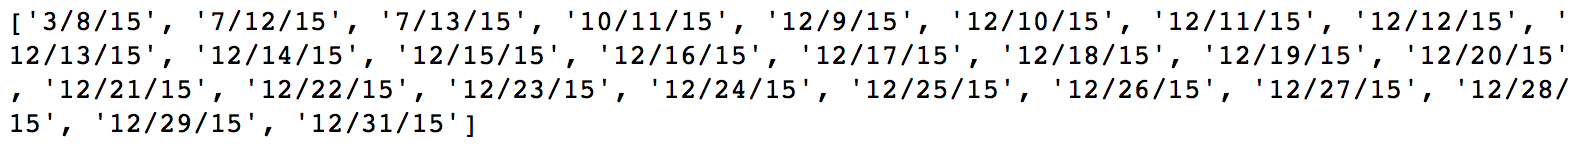
\includegraphics[width=\textwidth]{/home/saf537/Documents/CUSP/Capstone/Bus-Capstone/plots/missing_days}
\caption{Missing days in the dataset.}
\label{m_days}
\end{figure*}



From the list of missing days, December is the month with the most missing data, which contains 21 days without data. It is necessary to find out what factors cause this problem. If it is caused by some uncontrollable factors such as weather, some mitigation plan may be devised. But if it is caused by some human factors of systems factors, it should be avoided in the future.
      
\subsubsection*{Visualization of records throughout the year}
      
The total number of bus records by date are shown in Figure \ref{m_alldays}.



\begin{figure*}[!t]
  
  \label{m_alldays}
  \centering
    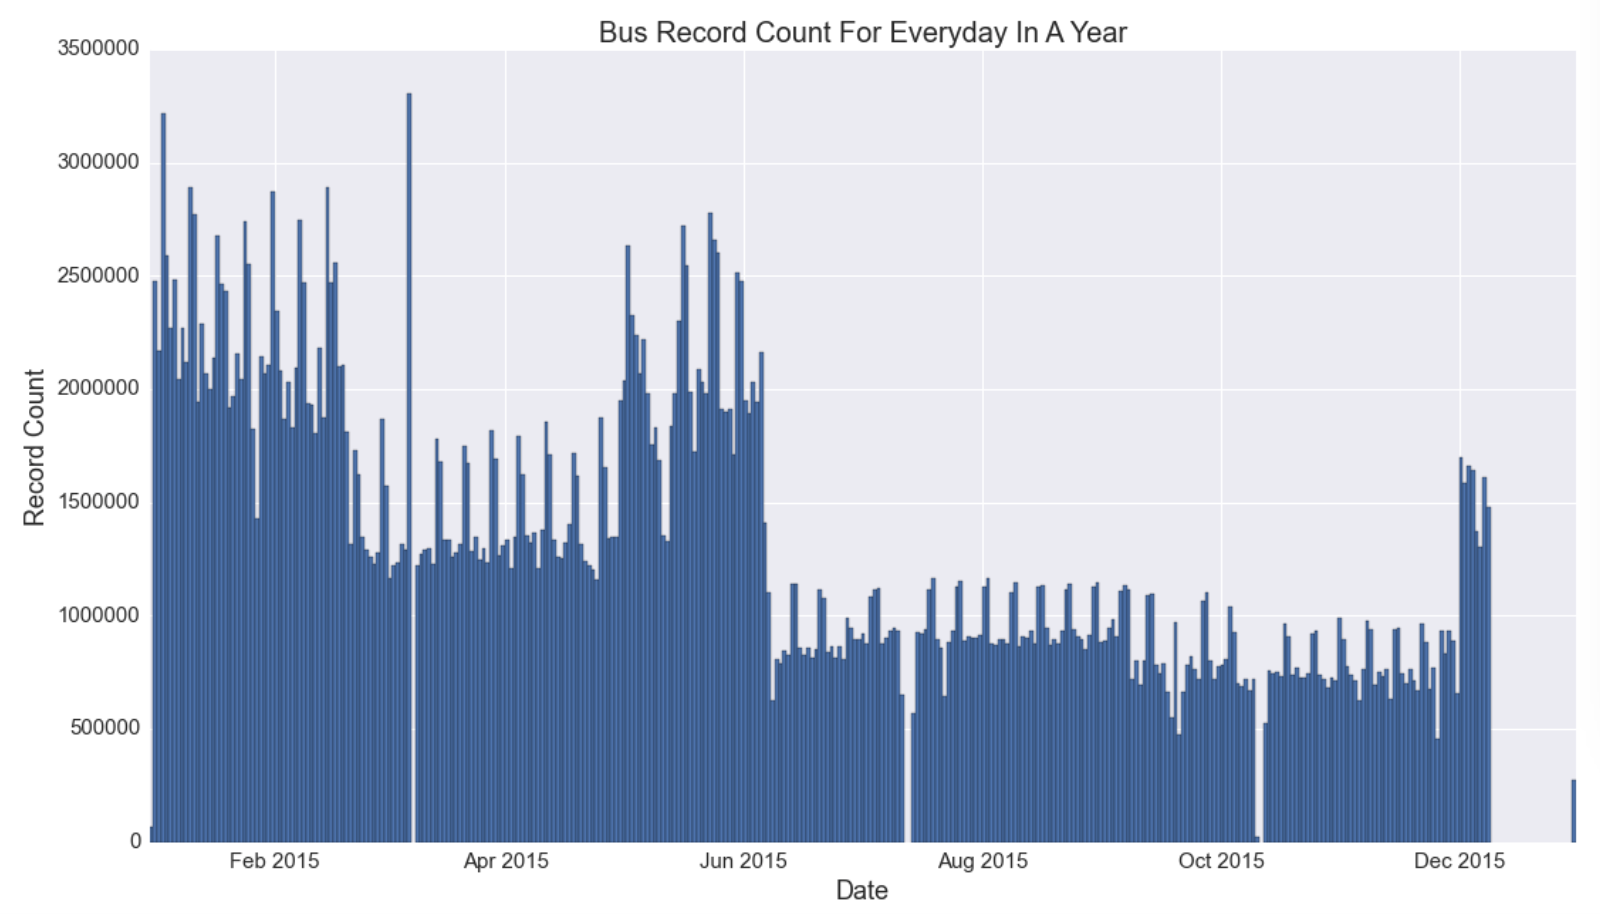
\includegraphics[width=\textwidth]{/home/saf537/Documents/CUSP/Capstone/Bus-Capstone/plots/whole_year_record}
    \caption{Visualization of records throughout the year.}
\end{figure*}

From the plot, some regularities are immediately apparent, including the seven-day cycle. However there are four obvious changes throughout the year. The first one is in February, second in May, third in June, and the last one in December. Further analysis is needed to find out these factors affecting the changes and could help with the bus schedule planning. Also, it can find that March 7th has an extremely high record but March 8th is a day without data which do not exist in other missing days. One can infer that data for March 8th were merged with March 7th.
      
      \subsubsection*{Daily record counts by hour}
      

\begin{figure*}[!t]
	\label{week}
  
  \centering
    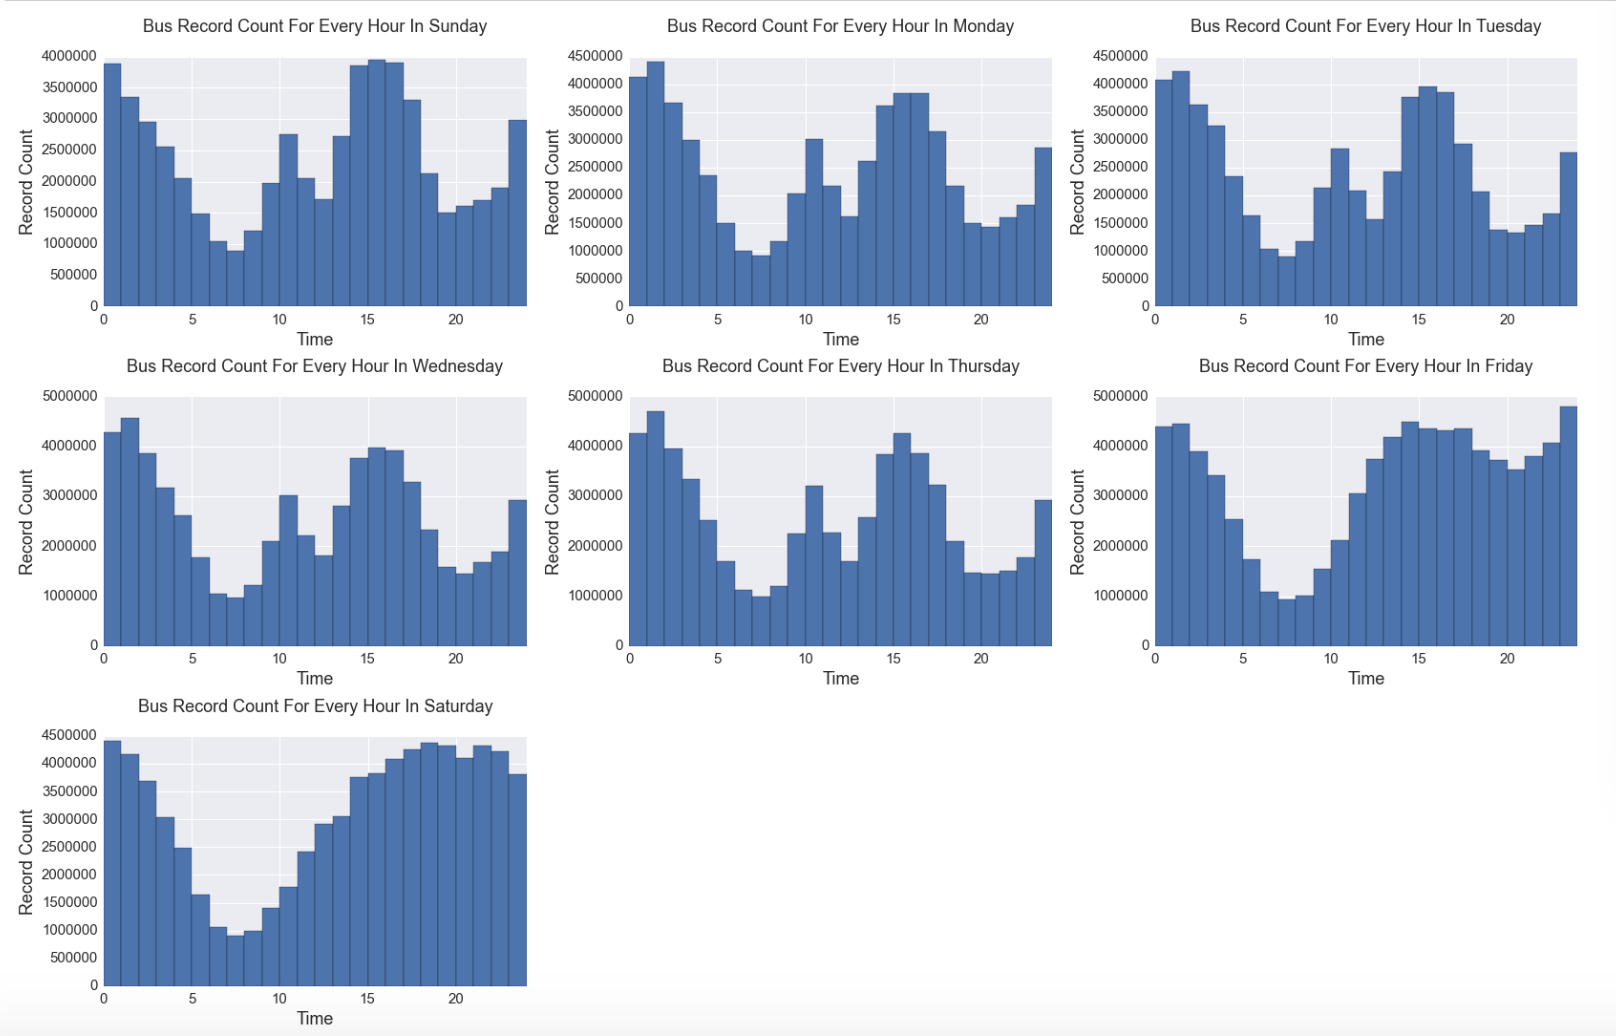
\includegraphics[width=\textwidth]{/home/saf537/Documents/CUSP/Capstone/Bus-Capstone/plots/whole_day_record}
    \caption{Bus records count for day of the week in 2015.}
\end{figure*}

From the plot, it can find that weekdays have the same trend and weekends have the same trend.   On weekdays, the record count regularly decreases as the morning progresses before peaking twice in the middle of the day.  In fact, one would expect the opposite based on typical characteristics of urban mobility: one peak during the morning rush-hour and one during the evening rush-hour.


      \subsubsection*{Data density with respect to level of scheduled activity}
      
       
   As the bus is transmitting every 30 seconds, the interval between Bus Time records is expected to also be 30 seconds so long as the vehicle is operating with the AVL equipment activated.  Figure 4 shows the actual intervals from the dataset collected.  In fact the typical interval turns out to be 60 seconds, with a significant portion of even longer intervals.  We examine these long intervals by comparing a measurement of total vehicle activity between the Bus Time data (in terms of record count) and the schedule data (in terms of aggregate running time of all scheduled trips). The measured activity from the two sources turn out to be strongly anticorrelated in the months analyzed (in the table below), whenever materially non-zero.  In other words, generally when scheduled activity increases, the density of data available in our dataset decreases.
   
\vspace{0.5cm}   
   
\resizebox{\columnwidth}{!}{
\begin{tabular}{l l l l l l l l l l}
\hline
Jan & Feb & Mar & Apr & May & Jun & Jul & Aug & Sep & Oct \\
\hline
-0.83 & -0.49 & -0.63 & -0.72 & -0.60 & 0.08 & -0.61 & -0.97 & -0.52 & 0.02 \\
\hline
\end{tabular}
}

\vspace{0.5 cm}

To further diagnose the issue, the comparison is made on a finer temporal scale (6-minute timesteps) for a few random dates.  Figure 5 shows very different patterns when overlaying the level of scheduled activity onto the level of reported activity derived from the Bus Time data.  On one of the two weekdays examined  (the first and third), two large gaps are clearly visible and span the entirety of the two daily rush-hour peaks in the schedule.  On the weekend date examined, a short gap is visible in the late evening.

The time series analysis showing counter-cyclical data density, the strong anticorrelation, and the tactical examination of a few dates all lead to the conclusion that the dataset collected by NYU CUSP cannot be used for performance analysis of an entire year without major risks to accuracy, in the form of both bias (as discussed in section 0.3.5: Arrival time estimation techniques) and variance (due to the most typical interval being twice as long as specified by MTA).  To continue with the demonstration of applying the data for performance metrics, we identified a week with the best density and limited gaps during rush hours (2015-12-01 to 2015-12-07).     
        
\begin{figure}[!t]
	\label{intervals}
  	
  	\centering
    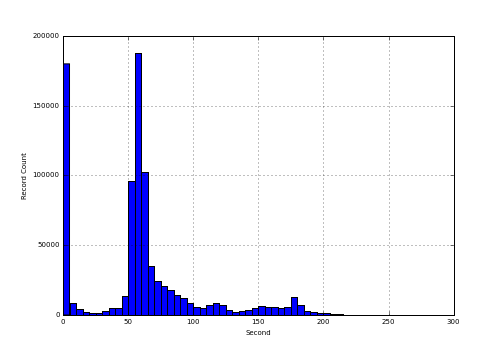
\includegraphics[width=\columnwidth]{/home/saf537/Documents/CUSP/Capstone/Bus-Capstone/plots/interva_distribution}
    \caption{Distribution of intervals between SIRI response records.}
\end{figure}

\begin{figure*}[!t]
	\label{trio}

  	\centering
    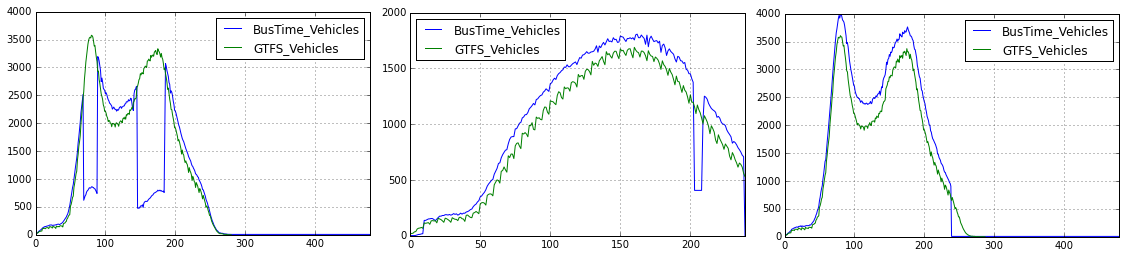
\includegraphics[width=\textwidth]{/home/saf537/Documents/CUSP/Capstone/Bus-Capstone/plots/trip_coverage_trio}
     \caption{Comparison of active vehicle count for three example dates.}
\end{figure*}


\subsubsection*{Tactical validation of individual elements}


Coordinates estimated using the Global Position System include some level of noise due to factors such as atmospheric conditions and multi-path effects. However the location elements of the Bus Time data appear to be transformed to adhere to shapelines of the reported bus route, eliminating any variation laterally across the street. Figure \ref{b26} shows an overlay of points from both Bus Time records and GTFS shape file data, for a short stretch of the B26 route in Fort Greene.  While the coordinates of stops are on the sides of the street, no lateral variation is observable in the Bus Time coordinates, even though the vehicles are known to travel along all four lanes of that specific roadway. Some error may remain along the orthogonal plane (the basis for distance calculations), but GPS-assistive equipment installed after the initial launch of Bus Time uses gyroscopes and speedometer readings to reduce this error to an immaterial level.

\begin{figure*}[!t]
\label{b26}
  
  \centering
    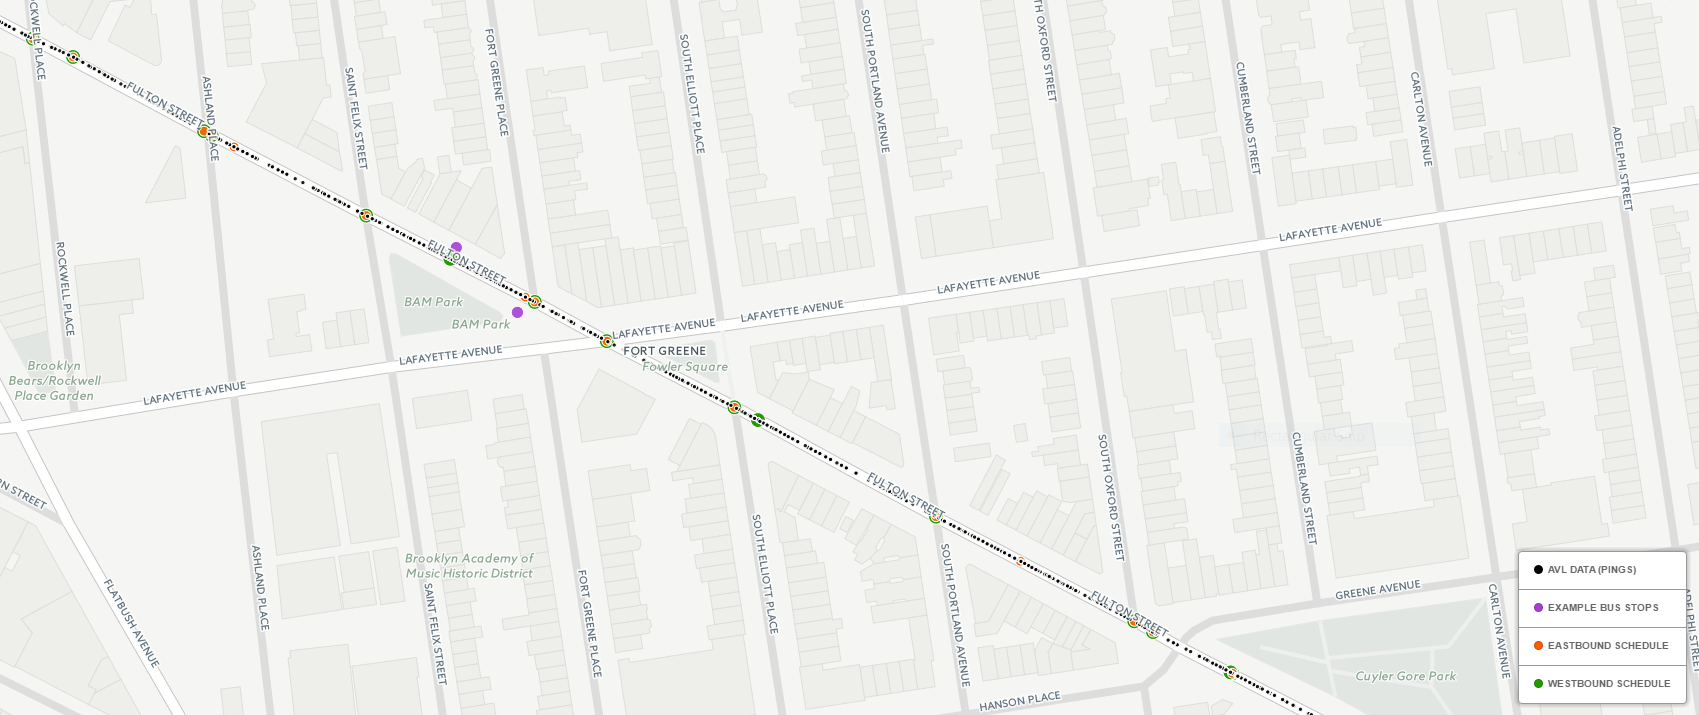
\includegraphics[width=\textwidth]{/home/saf537/Documents/CUSP/Capstone/Bus-Capstone/plots/b25_detail}
    \caption{Sample of B25 route.}
\end{figure*}

The only elements reported by the vehicle itself are the time, location and headsign (the route and destination text displayed above the front of the vehicle).  All of the remaining elements are inferred by the Bus Time server.  Because those inferences are made real-time, the software has no opportunity to retrospectively validate and correct errors.  This analysis validates two key features by checking for two metadata properties: that reported trip IDs are unique to each vehicle and that stop distances are unique for each shape.  The first validation failed while the second property was confirmed.  Figure 7 is a sample summary of records records grouped by both trip and vehicle, for a sample date and route; it shows the duplication of trip ID across multiple vehicles, the number of records associate with each duplicate, and the timespan of those records.

%
\begin{figure*}[!t]
\label{trip_val}
  
  \centering
    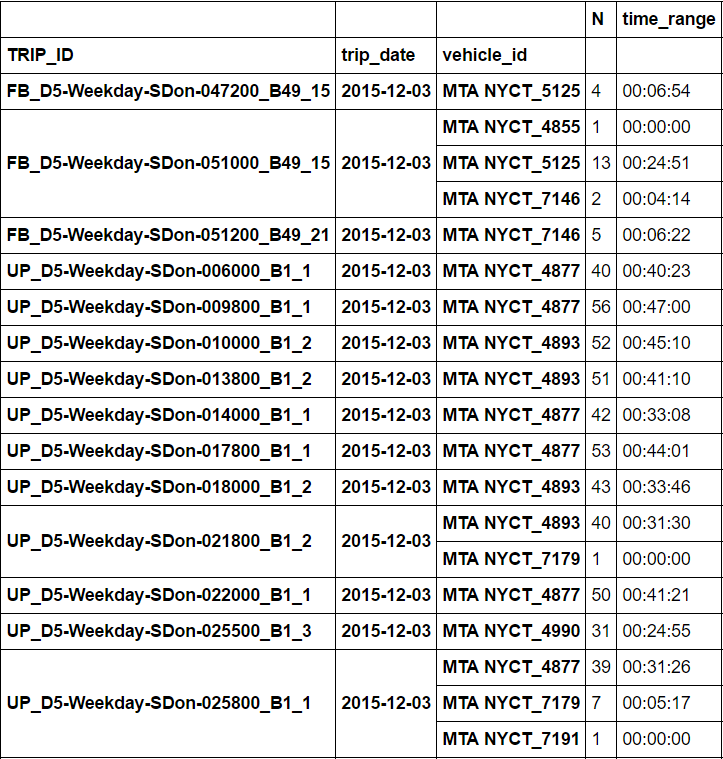
\includegraphics[width=\textwidth]{/home/saf537/Documents/CUSP/Capstone/Bus-Capstone/plots/trip_vehicle_validation}
    \caption{Duplication of Trip ID across several vehicles}
\end{figure*}

The conclusions are that the Bus Time server sometimes makes errors in inference of the vehicle's trip ID, the inferred trip ID is not persistent for a vehicle (that is, it "flip flops"), but the reported stop distances for the inferred shape are persistent.  The variation in inferred trip ID is an important consideration in subsequent performance measurement because so much of the analysis requires grouping or sorting data (both input and output) by trip.




\subsection{Demonstrations of the methods applied to the dataset}

The practices of transportation planning and analysis rely heavily on vehicle arrival-time data. The first phase of this report explained the retrieval of real-time AVL data and application of methods for estimating those arrival times in actual operations. The following list demonstrates some typical analytic techniques and discusses their validity when applying these data, given the known limitations to its density and accuracy. Included in the input data are arrival times from the schedule, published in the widely-adopted General Transit Feed Specification, but discussion of its data generation process is not in scope. Generally, many high-level performance metrics are simple ratios expressing the proportion of events (such as a vehicle arrival, or completed trip) that meet some criteria (such as arriving within 5 minutes of its scheduled time). The problem with these binary measurements is that the methods ignore the shape (referred to in mathematics as higher moments) of a distribution - for example, a "long tail," or if the distribution is multi-modal.

\begin{itemize}
\item \textbf{Distribution of headway}: In higher-frequency transit routes, arrivals are considered reliable when the headway is more consistent and closer to customers' expectation.  (The ideal distribution is 100\% density at the expected value, that is, no deviation.  Our definition of Headway Adherence is binary and allows for some deviation).  The distribution of headway for a less-than-reliable service is not always a normal bell-curve.  This is because of the tendency for delayed buses to become even more delayed, as the larger number of waiting passengers increases dwell times, which in turn reduces overall travel speed.  When bunching occurs, the headways of the "bunched" buses (i.e., those that closely follow a preceding delayed bus) approach zero, while there is no theoretical upper limit for the headway of the delayed bus.
\item \textbf{Bunching rate}: Variations in dwell time and variations between-stop travel time related to traffic and operator behavior are the major causes of vehicle bunching along a route (Gellei 2010).  Measurement of dwell time and travel time will be discussed later in this section.  The resulting bunching condition can be measured.  For this analysis, we consider the bunching condition to occur when headway is less than one minute.  The bunching ratio is the percentage, at a certain stop, of arrivals under bunching condition compared to total vehicle arrivals.  This is very similar to Headway Adherence except that it measures the tail of the distribution, not the middle.  Bunching ratio can be calculated and compared for a variety of stops and routes, as shown in Figure \ref{bunch}.


\begin{figure*}[!t]

  \label{bunch}
  \centering
    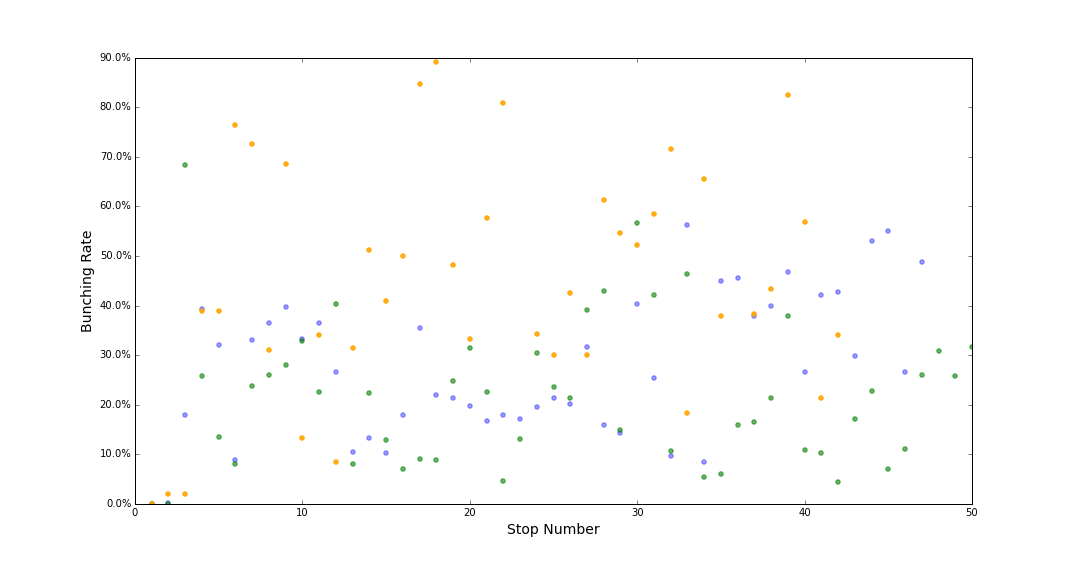
\includegraphics[width=\textwidth]{/home/saf537/Documents/CUSP/Capstone/Bus-Capstone/plots/bunching_rates}
      \caption{Headway Bunching Rate at Stops for Three Brooklyn Bus Routes.}
\end{figure*}



\item \textbf{Distribution of running time adherence:} Best practice in schedule planning is to forecast running time using historical data, but exclude outliers. An outlier often represents an occurrence of some enroute incident (such as a police action or a parade) and should not influence planning a typical-day bus schedule. Outliers skew upward the distribution of actual running times, since there is a physical upper limit to the vehicle's speed, but no limit to the number and severity of enroute incidents. Because the schedules are created based on historical distributions excluding outliers, the resulting error, defined as running time variance, will tend to be positive. The error can be mitigated by artificially increasing the planned running time (for example, by including the outliers, or adding some arbitrary value), but it is generally not cost- effective to do so, or impacts the reliability of subsequent trips operated by the same vehicle or operator.


One example descriptive analysis is to plot the distribution of normalized running time variances. Visible in this example, Figure \ref{adh}, is both the central tendency -- slightly positive -- and the wide spread of the distribution, indicating very inconsistent running time adherence.  Strategies to reduce the inconsistency are not in the scope of this project.




\begin{figure*}[!t]

  \label{adh}
  \centering
    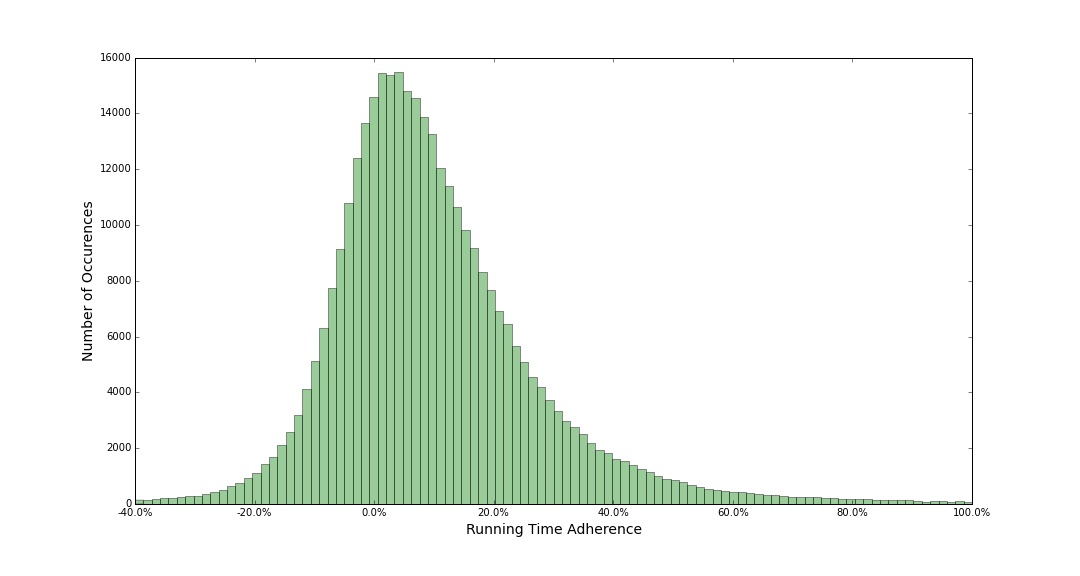
\includegraphics[width=\textwidth]{/home/saf537/Documents/CUSP/Capstone/Bus-Capstone/plots/running_time_adherence}
      \caption{Running time adherence.}
\end{figure*}


\item \textbf{Performance with respect to vehicle distance along route:} It is generally accepted in the theory of urban public transportation that longer routes have worse reliability, as defined by the metrics discussed so far.  Another analytic technique is to plot one of the metrics for a given route (or, more specifically - one shape variation of a route). Figure \ref{ols} is the summary of an ordinary least squares (OLS) regression, taking Wait Assessment as the dependent variable and the vehicle's progression along the shape (in terms of number of stops made) as the independent variable.  The resulting parameter value has strong statistical significance, rejecting the null hypothesis that route length has no relationship to performance.  The example in Figure \ref{wastop} both supports that conclusion and suggests which segments along the route contribute most to the decline.

\begin{figure*}[!t]
  
  \label{ols}
  \centering
    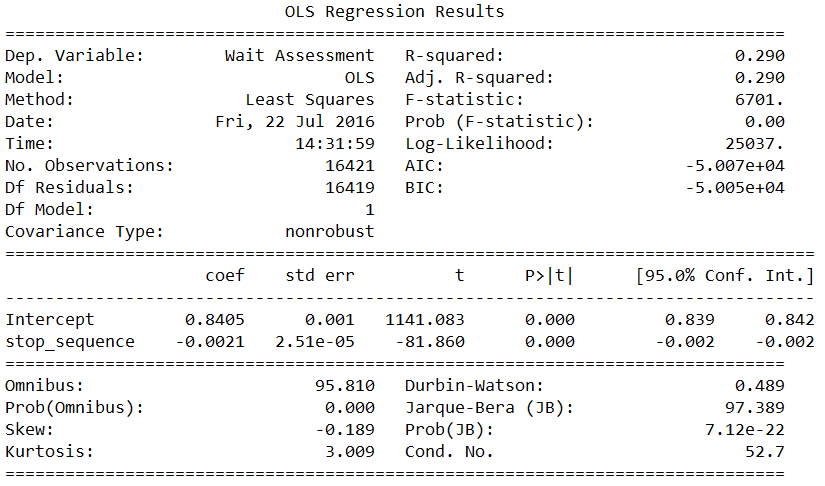
\includegraphics[width=\textwidth]{/home/saf537/Documents/CUSP/Capstone/Bus-Capstone/plots/ols_summary}
    \caption{Correlation of Wait Assessment and Stop Sequence Number.}
\end{figure*}


\begin{figure}[!t]
  \label{wastop}
  \centering
    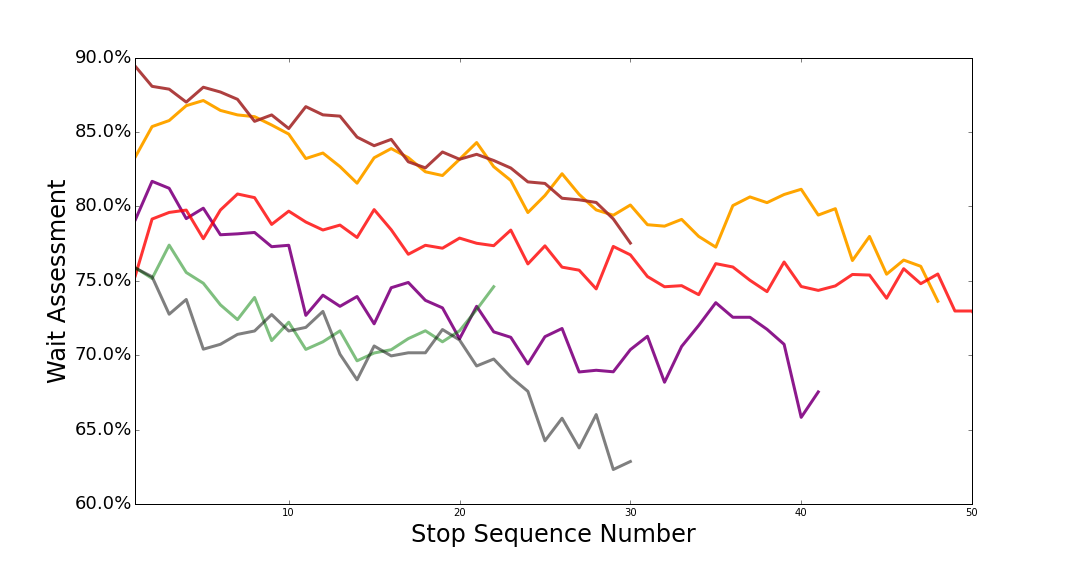
\includegraphics[width=\columnwidth]{/home/saf537/Documents/CUSP/Capstone/Bus-Capstone/plots/wa_by_stop_sequence}
      \caption{Average Wait Assessment by Stop Sequence Number, Route B41.}
\end{figure}

\vspace{0.5cm}

\item \textbf{Spatial distribution of travel speeds:} Because Bus Time records contain discrete time and location, speed calculations are difference-based averages, not instantaneous (or quasi-instantaneous) samples.  The other challenge in descriptive statistics about speed at fixed location(s) is that the sequential observation points of multiple vehicles are not aligned; for example it is extremely unlikely that multiple vehicles record the "ping" from exactly 100 meters and again at exactly 200 meters along a route-shape.  However re-sampling is possible if mean speeds are treated as continuous curves with respect to distance.  The new distribution at a point is defined as the collection of mean speeds of all vehicles passing that point.  \ref{msd} demonstrates the changing moments of the distribution over the length of a route-shape, along with grid lines indicating the stop locations.

\begin{center}
\begin{figure}[!t]
  
  \label{msd}
  \centering
    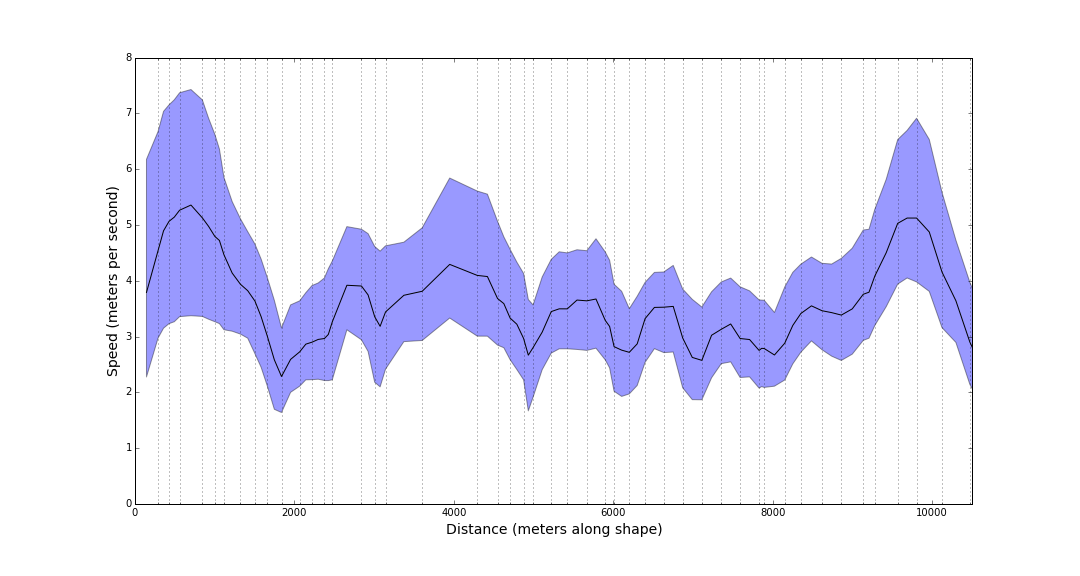
\includegraphics[width=\columnwidth]{/home/saf537/Documents/CUSP/Capstone/Bus-Capstone/plots/moving_speed_distribution}
    \caption{Moving speed distribution.}
\end{figure}
\end{center}

\item \textbf{Spatial distribution of slow/stopped condition} - A list of slow/stopped events can be created by identifying the beginning and end location and times for each occurrence of the condition.  Naturally, many of these events will be at stop locations.   That subset of the slow/stopped events may theoretically support analysis of dwell time, however even when using data having the maximum density possible according the data generation process (every 30 seconds), analysis of dwell time at individual stops is not possible; previous research suggests that the majority of stops have dwell time of less than 30 seconds (Pangilinan 2011).  The remaining subset are slow/stopped events not occurring at stop locations.  High spatial density of these events indicates a recurring problem with traffic flow, which in turn increases travel time and contributes to occurrence of bunching condition.  (In order to exclude the normal interaction with traffic signals, the events can be filtered to only include those above some minimum, related to traffic signal cycle lengths).

Figure \ref{stopped_slow} shows the estimated percentage of vehicles in slow/stopped condition and many points along a route-shape.  While some extreme values are apparent, they are generally at stop locations and the variance of the remaining points is minimal, even at other stop locations.  This suggests that the density of the data may be insufficient to identify interruptions without a high rate of false negatives.



\begin{figure}[!t]
  
  \label{stopped_slow}
  \centering
    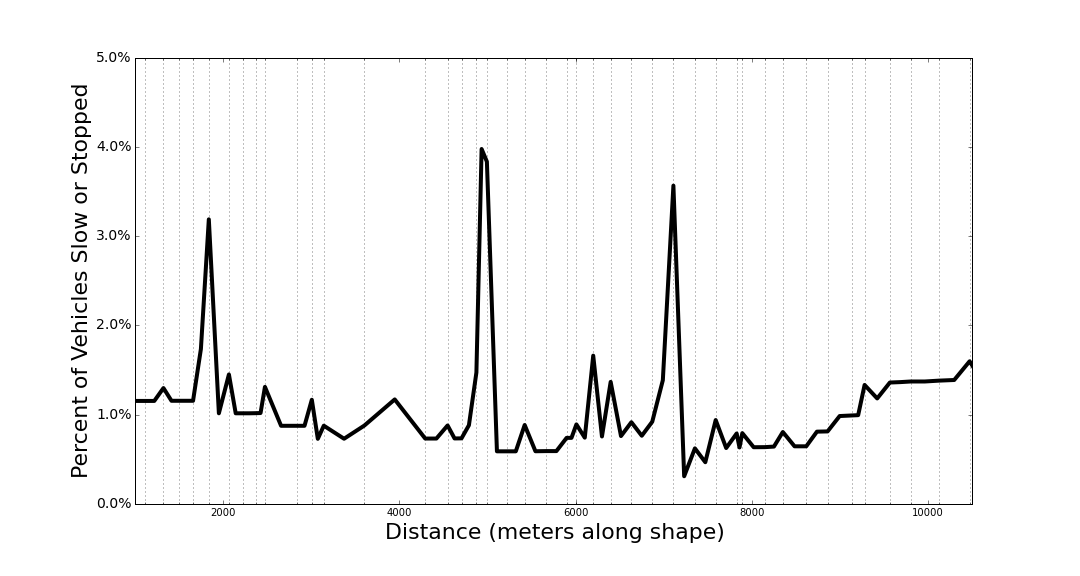
\includegraphics[width=\columnwidth]{/home/saf537/Documents/CUSP/Capstone/Bus-Capstone/plots/percent_vehicles_slow_or_stopped}
    \caption{Stopped or Slow Vehicle Percentage.}
\end{figure}




\end{itemize}


\section{Limitations of the analysis and future ways to address them}

\subsection{Data}


On the one hand, the huge size of data requires big data techniques. The biggest challenge for our approach to be implemented in practice by cities is that of processing large amounts of raw data into information because it requires big data techniques for anything beyond small samples (i.e. one line, one day, etc.). Even processed datasets being structured can demand more than what can be offered by single/dual core applications. Data supporting higher-level analysis techniques can be managed with any off-the-shelf database system, including \textit{sqLite} (open source SQL) or even a series of CSVs. Furthermore, the large amounts of data require a special environment to deal with. Since the raw data could not be dealt with in local machines because of its volume, we used CUSP's cluster and Data Facility to process it. 

It is worth noting that, while the MTA does not publish archived Bus Time data (except for a sample in 2014), we are providing the code for anybody to collect it, and this is an important step that must be kept into account when discussing about privacy. Besides this, the Vehicle
ID field is not anonymized, so the contributions of our project are subject to have unlikely yet feasible implications regarding tracking of individuals, to the extent they can be identified in a relatable data source.



\subsection{Accuracy}

Accuracy of the location and time data, when reported, was not in question for the purposes of this project. However, some of the elements are inferred and may cause errors if not handled properly.
Limitations are generally the result of information gaps, specifically when no data is reported when or where expected. When no data is reported, it is unknown if there was actually an operating bus, but a problem arose with hardware or software. Also, if there was a bus (for example, present in previous and latter data points), it is possible that the bus did not follow the scheduled route. 

There are also some limitations from the data that ends up being recorded:

\begin{itemize}
\item There are trips with data from more than one vehicle, which means that trips use a combination of reported trip\_id and vehicle id.
\item Uncertainty in dwell time.
\item Lack of instantaneous speed information.
\item Lack of schedule meta data.
\item Since the system automatically infers trips and stations, there are signals showing disappearing and reappearing buses.
\end{itemize}


\subsection{Frequency}

The ideal interval for every continuous collected time stamp is 30 seconds. But there exists a large amount of data points intervals over 30 seconds or even over an hour. That may be due to delays in signal collection. 

In order to analyse both the vehicle behaviour on individual street segments and intersections, and the dwell times, 60-90 second frequency is insufficient. Thirty seconds are also insufficient for the measurement of dwell time.

As the interval can not be change or fix in the dataset, this project reported this situation. Alos, as the dataset contain a whole year information, the trend and regularity can be obvious even though the interval is not within 30 seconds. In the future analysis, if GPS can get a more accurate data collecting, that will make the project analysis more accurate. Bus travelling data is necessary for future DOT planning decisions and bus behaviors analyzing.In order to improve the data collecting process, it could improve the sensibility of sensors. 
\subsection{Gaps}
Frequent, long gaps in the data make unbiased performance analysis impossible over full days or date ranges, because the gaps tend to arise at the same times each day. Any statistical measurement involve time-of-day as an input variable will be biased. Some analysis may leave time-of-day as an unobserved component of the error term and still show significance in other variables, such as distance-along-trip or street features.
Incomplete reporting of trips may cause bias in calculation of trip-based measurements, such as running time and On Time Performance, if not normalized. Just as mentioned in Accuracy sections, over-30-second interval may affect the accuracy of the analysis.
Inferences of points beyond the range of data need to be flagged specially given the possibility that the vehicle did not operate the trip as planned. If better density is useful, DOT should request the additional elements in the static files provided by MTA

\subsection{Tecnology}

As the dataset for this project is extremely huge, the only way to make the process more faster is using big data technology. That would need the help of CUSP data facilities.So the main advantages of our approach rely on the fact that it is based on open source software (such as Python, HDFS and Spark) with a wide and increasing support community around them, but also on the fact that our code is simple to share and reproduce. Since Big Data software is relatively new, we kept most of the data manipulation in simple SQL or Python scripts, which is specially convenient for the client.


\subsection{Reproducibility}

The main risk identified by our approach is reproducibility in terms of data fetching and of framework dependency. Our data feed depends on a public API that is always subject to interruptions, and the Big Data processing requires the HDFS management system and Spark. It may take time and computational and technical resources to handle them, and deprecation is always a hazard. Despite of this, those potential sources of failure have been proven to be increasing in robustness and trustworthiness during the last years.



\section{Conclusions and future research}

\subsection{Conclusions}

This project studies the possibility of calculating performance metrics for bus performance in New York City based on the GPS data offered by MTA. The MTA bus GPS database collects the location of each bus every 30 seconds. After estimating the departure and arrival time for each bus at each stop, we use measurement like headways and wait assessment to assess bus performance and reliability. Taking one-year data as our object of study, the data is extremely huge so that big data techniques (mainly Spark) are widely used in this project. In order to make our work easy to share and reproduce, we choose to use the SQL API to decide on the parsing of the data, which enables the DOT to easily make changes by editing the SQL script.
Positive aspects of our approach include the fact that we focused this analysis on the viewpoint of the DOT; the fact that we were able to successfully process large volumes of data; the fact that we identified pitfalls and challenges of using the MTA Bus Time data for the purposes of the sponsor agency and the fact that we enable a flexible implementation of different methods to estimate times and locations, as well as to measure schedule-reliability performance.
Potential pitfalls and areas of improvement are the fact that we used formal metrics that were not tailored for the DOT nor New York City, and the abundance of assumptions that inevitably scale up, both with and without bias, in the form of measurement errors.
Similar methodologies and concepts could be used in other cities and traffic models. The big data technology applied in not only traffic analysis but also city wide urban issue offers more reliable results compared with traditional sample studies.


\subsection{Recommendations to DOT}

Use of the public API for real-time archiving of Bus Time data mimics an ongoing process already performed internally at MTA, and can result in an incomplete view of the same data.  Moreover, the static file currently used by DOT, presumably provided by MTA, contains both greater temporal density and some additional, potentially useful elements that are not available through the Bus Time API.  The results of this project suggest that combining the advantages of both data acquisition processes would yield the ideal dataset needed for these analyses.  The DOT may request that MTA include the additional, useful vehicle monitoring elements in the file provided directly to DOT and therefore eliminate temporal gaps that arise due to problems with the public API.
The subsequent interpolation and performance analysis steps do not require the user to implement a so-called big data platform if Bus Time data is processed in smaller batches (for example, one full day) as it accumulates.  Once headway, running time, and vehicle speed calculations are performed and output stored with proper indexing, the performance metrics can be dynamically analyzed using a typical personal computer.

\subsection{Suggestions for future work}

\begin{itemize}
\item Inference study of the effect of several traffic or design conditions on reliability.
\item Autocorrelation to identify recurring patterns in reliability with respect to time (for example, every Monday morning)
\item  Integrate and Improve the current visualization tool developed by NYU CUSP, and adapt it to be responsive and interactive to different queries.

\item Further optimize the algorithms hereby used for the Big Data portion of the work.
\item Generalization of code for further applications:
\begin{itemize}
\item Other transit system data feeds may use a different interface standard and as a result a different data structure-   AVL systems in some cities collect stop departure and arrival time directly, instead of location at fixed time intervals).
\item Other transit modes, for example subway or bike-share,  may contain different features specific to that mode.
\end{itemize}
\end{itemize}

\section*{Author contributions}

All authors work contributed extensively to the work presented in this paper with discussions and communications with mentors and sponsor. 
Matthew P Urbanek extracted the data using MTA BusTime API and did the data quality analysis for the whole year data with Bonan Yuan. Sara Arango is responsible for the arrival time interpolation. Bonan Yuan parsed all the extracted data from the whole year json files and processed the analysis on the large dataset by Spark. Yuqiao Cen did the gap record analysis. Jiaxu Zhou developed the performance assessment metrics. 






% Can use something like this to put references on a page
% by themselves when using endfloat and the captionsoff option.
\ifCLASSOPTIONcaptionsoff
  \newpage
\fi



% trigger a \newpage just before the given reference
% number - used to balance the columns on the last page
% adjust value as needed - may need to be readjusted if
% the document is modified later
%\IEEEtriggeratref{8}
% The "triggered" command can be changed if desired:
%\IEEEtriggercmd{\enlargethispage{-5in}}

% references section

% can use a bibliography generated by BibTeX as a .bbl file
% BibTeX documentation can be easily obtained at:
% http://www.ctan.org/tex-archive/biblio/bibtex/contrib/doc/
% The IEEEtran BibTeX style support page is at:
% http://www.michaelshell.org/tex/ieeetran/bibtex/
%\bibliographystyle{IEEEtran}
% argument is your BibTeX string definitions and bibliography database(s)
%\bibliography{IEEEabrv,../bib/paper}
%
% <OR> manually copy in the resultant .bbl file
% set second argument of \begin to the number of references
% (used to reserve space for the reference number labels box)
\begin{thebibliography}{14}

\bibitem{Lin}
W. H. Lin and J. Zeng, "An experimental study of real-time bus arrival time prediction with GPS data," Transp. Res. Rec., no. 1666, pp. 101- 109, Jan. 1999.

\bibitem{Raj}
Rajat Rajbhandari, Steven I. Chien, and Janice R. Daniel, ''Estimation of bus dwell times with APC information'', Transportation Research Record 1841 Paper No. 03- 2675, 2003.

\bibitem{Min-Tang}
Min-Tang Li, Fang Zhao, Lee-Fang Chow, Haitao Zhang, and Shi-Chiang Li, ''Simulation Model for Estimating Bus Dwell Time by Simultaneously Considering Numbers of Disembarking and Boarding Passengers'', Transportation Research Record 1971, 2006.

\bibitem{Fazhi}
LI Fazhi, Yang Dongyuan, and Ma Kai, ''Bus Rapid Transit (BRT) Bunching Analysis With Massive GPS Data,'' National Science and Technology Support Program of China (NO. 2009BAG17B01), 2013.

\bibitem{Levine}
Brian Levine, Alex Lu, and Alla Reddy, ''Measuring Subway Service Performance at New York City Transit: A Case Study Using Automated Train Supervision (ATS) Track-Occupancy Data,'' TRB 2013 Annual Meeting, 2013.

\bibitem{DanWan}
Dan Wan, Camille Kamga, Jun Liu, Aaron Sugiura, and Eric B. Beaton, ''Rider perception of a ‘light' Bus Rapid Transit system - The New York City Select Bus Service,'' Transport Policy 49 (2016) 41–55, Apr. 2016.

\bibitem{Bie}

Yiming Bie, Xiaolin Gong, and Zhiyuan Liu, ''Time of day intervals partition for bus schedule using GPS data,'' Transportation Research Part C 60, pp. 443–456, Sep. 2015.

\bibitem{Safran}
Jeremy S. Safran, Eric B. Beaton, and Robert Thompson, ''Factors Contributing to Bus Lane Obstruction and Usage in NYC: Does Design Matter?'' TRB 2014 Annual Meeting, 2014

\bibitem{Pangil}
Christopher Pangilinan, Nigel Wilson, and Angela Moore, ''Bus Supervision Deployment Strategies and Use of Real-Time Automatic
Vehicle Location for Improved Bus Service Reliability,'' Transportation Research Record: Journal of the Transportation Research Board, No. 2063, Transportation Research Board of the National Academies, Washington, D.C., 2008, pp. 28–33. DOI: 10.3141/2063-04.

\bibitem{Yang}
Yingxiang Yang, David Gerstle, Peter Widhalm, and Dietmar Bauer, ''The Potential of Low-Frequency AVL Data for the Monitoring and Control of Bus Performance,'' TRB 2013 Annual Meeting, 2013.

\bibitem{ShiAn}
Shi An, Xinming Zhang and Jian Wang, ''Finding Causes of Irregular Headways Integrating Data Mining and AHP,'' ISPRS Int. J. Geo-Inf. 2015, 4, 2604-2618; DOI:10.3390/ijgi4042604, Nov. 2015.

\bibitem{Jinil}
Jinil Chang, Mohamad Tala, and Satya Muthuswamy, ''A Simple Methodology To Estimate Queue Lengths at Signalized Intersections Using Detector Data,'' TRB 2013 Annual Meeting, 2013.

\bibitem{Chris}
Christopher Pangilinan and Kristen Carnarius, ''Traffic Signal Timing for Optimal Transit Progression in Downtown San Francisco,'' San Francisco Municipal Transportation Agency, San Francisco, CA, 2011.

\bibitem{Reed}
Simon Reed, ''Transport for London Using Tools, Analytics and Data to Inform Passengers,'' JOURNEYS, September 2013. \url{https://www.lta.gov.sg/ltaacademy/doc/13Sep096-Reed_TfL-InformPassengers.pdf}, accessed 20 Jul 2016.

\end{thebibliography}


\onecolumn
\appendices
\section{Sample visualization}

\begin{figure*}[h!]
  \caption{On time performance aggregated by stop over 2015.}
  \centering
    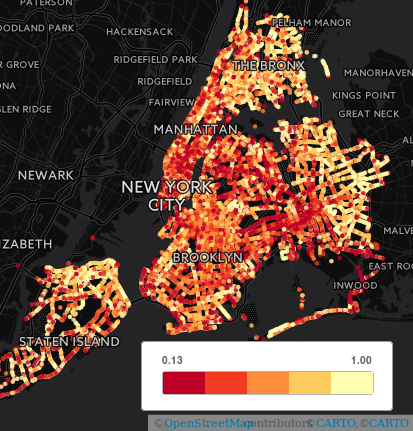
\includegraphics[width=\textwidth]{/home/saf537/Documents/CUSP/Capstone/Bus-Capstone/plots/on_time_performance_stops}
\end{figure*}

% biography section
% 
% If you have an EPS/PDF photo (graphicx package needed) extra braces are
% needed around the contents of the optional argument to biography to prevent
% the LaTeX parser from getting confused when it sees the complicated
% \includegraphics command within an optional argument. (You could create
% your own custom macro containing the \includegraphics command to make things
% simpler here.)
%\begin{IEEEbiography}[{\includegraphics[width=1in,height=1.25in,clip,keepaspectratio]{mshell}}]{Michael Shell}
% or if you just want to reserve a space for a photo:

%\begin{IEEEbiography}{Michael Shell}
%Biography text here.
%\end{IEEEbiography}

% if you will not have a photo at all:
%\begin{IEEEbiographynophoto}{John Doe}
%Biography text here.
%\end{IEEEbiographynophoto}

% insert where needed to balance the two columns on the last page with
% biographies
%\newpage

%\begin{IEEEbiographynophoto}{Jane Doe}
%Biography text here.
%\end{IEEEbiographynophoto}

% You can push biographies down or up by placing
% a \vfill before or after them. The appropriate
% use of \vfill depends on what kind of text is
% on the last page and whether or not the columns
% are being equalized.

%\vfill

% Can be used to pull up biographies so that the bottom of the last one
% is flush with the other column.
%\enlargethispage{-5in}



% that's all folks
\end{document}

